\documentclass[t]{beamer}
\usetheme[deutsch]{KIT}
\setbeamercovered{transparent}
\setbeamertemplate{navigation symbols}{}
\graphicspath{ {Systemmodelle/images_blank/} }

\KITfoot{ Croggle - Praxis der Softwareentwicklung WS 13/14}
\usepackage[utf8]{inputenc}
\usepackage{ngerman}
\usenavigationsymbols


\title{Croggle}
\subtitle{PSE - Planungsphase \\[0.3cm]
Lukas Böhm $\cdot$ Tobias Hornberger $\cdot$ Jonas Mehlhaus \\ Iris Mehrbrodt  $\cdot$ Vincent Schüßler $\cdot$ Lena Winter}
\institute[IPD]{Institut für Programmstruktutren und Datenorganisation}

\TitleImage[height=\titleimageht]{Banner.png}

\AtBeginSection[]
{
  \begin{frame}
    	\frametitle{Übersicht}
    	\tableofcontents[currentsection]
  \end{frame}
}

\begin{document}

\begin{frame}
        \maketitle
\end{frame}

\begin{frame}
        \frametitle{Übersicht}
        \addcontentsline{toc}{section}{}
        \tableofcontents
\end{frame}

\section{Zielsetzung}
\begin{frame}
	\frametitle{Vorgaben}
	Entwickeln einer Lernapplikation für Kinder:\\
	\begin{itemize}
		\item Zielgruppengerechte Bedienung
		\item Anhaltende Motivation
		\item Kontrolle des Lernfortschritts
	\end{itemize}
\end{frame}

\begin{frame}
	\frametitle{Spielprinzip}
	Spielidee von Bret Victor: \\
     \\
	\begin{itemize}
		\item Alligatoren repräsentieren die Abstraktionen im \(\lambda\)-Kalkül
		\item Eier stellen die Variablen des \(\lambda\)-Kalküls da
		\item Alte Alligatoren dienen zur Darstellung der Klammern
		\item Familien bestehen aus Eiern, Alligatoren, alten Aligatoren und anderen Familien 
	\end{itemize}
	
\includegraphics[width=\textwidth]{Spielelemente.png}
\end{frame}

\section{Umsetzung}
\begin{frame}
	\frametitle{Multiple-Choice Level}
	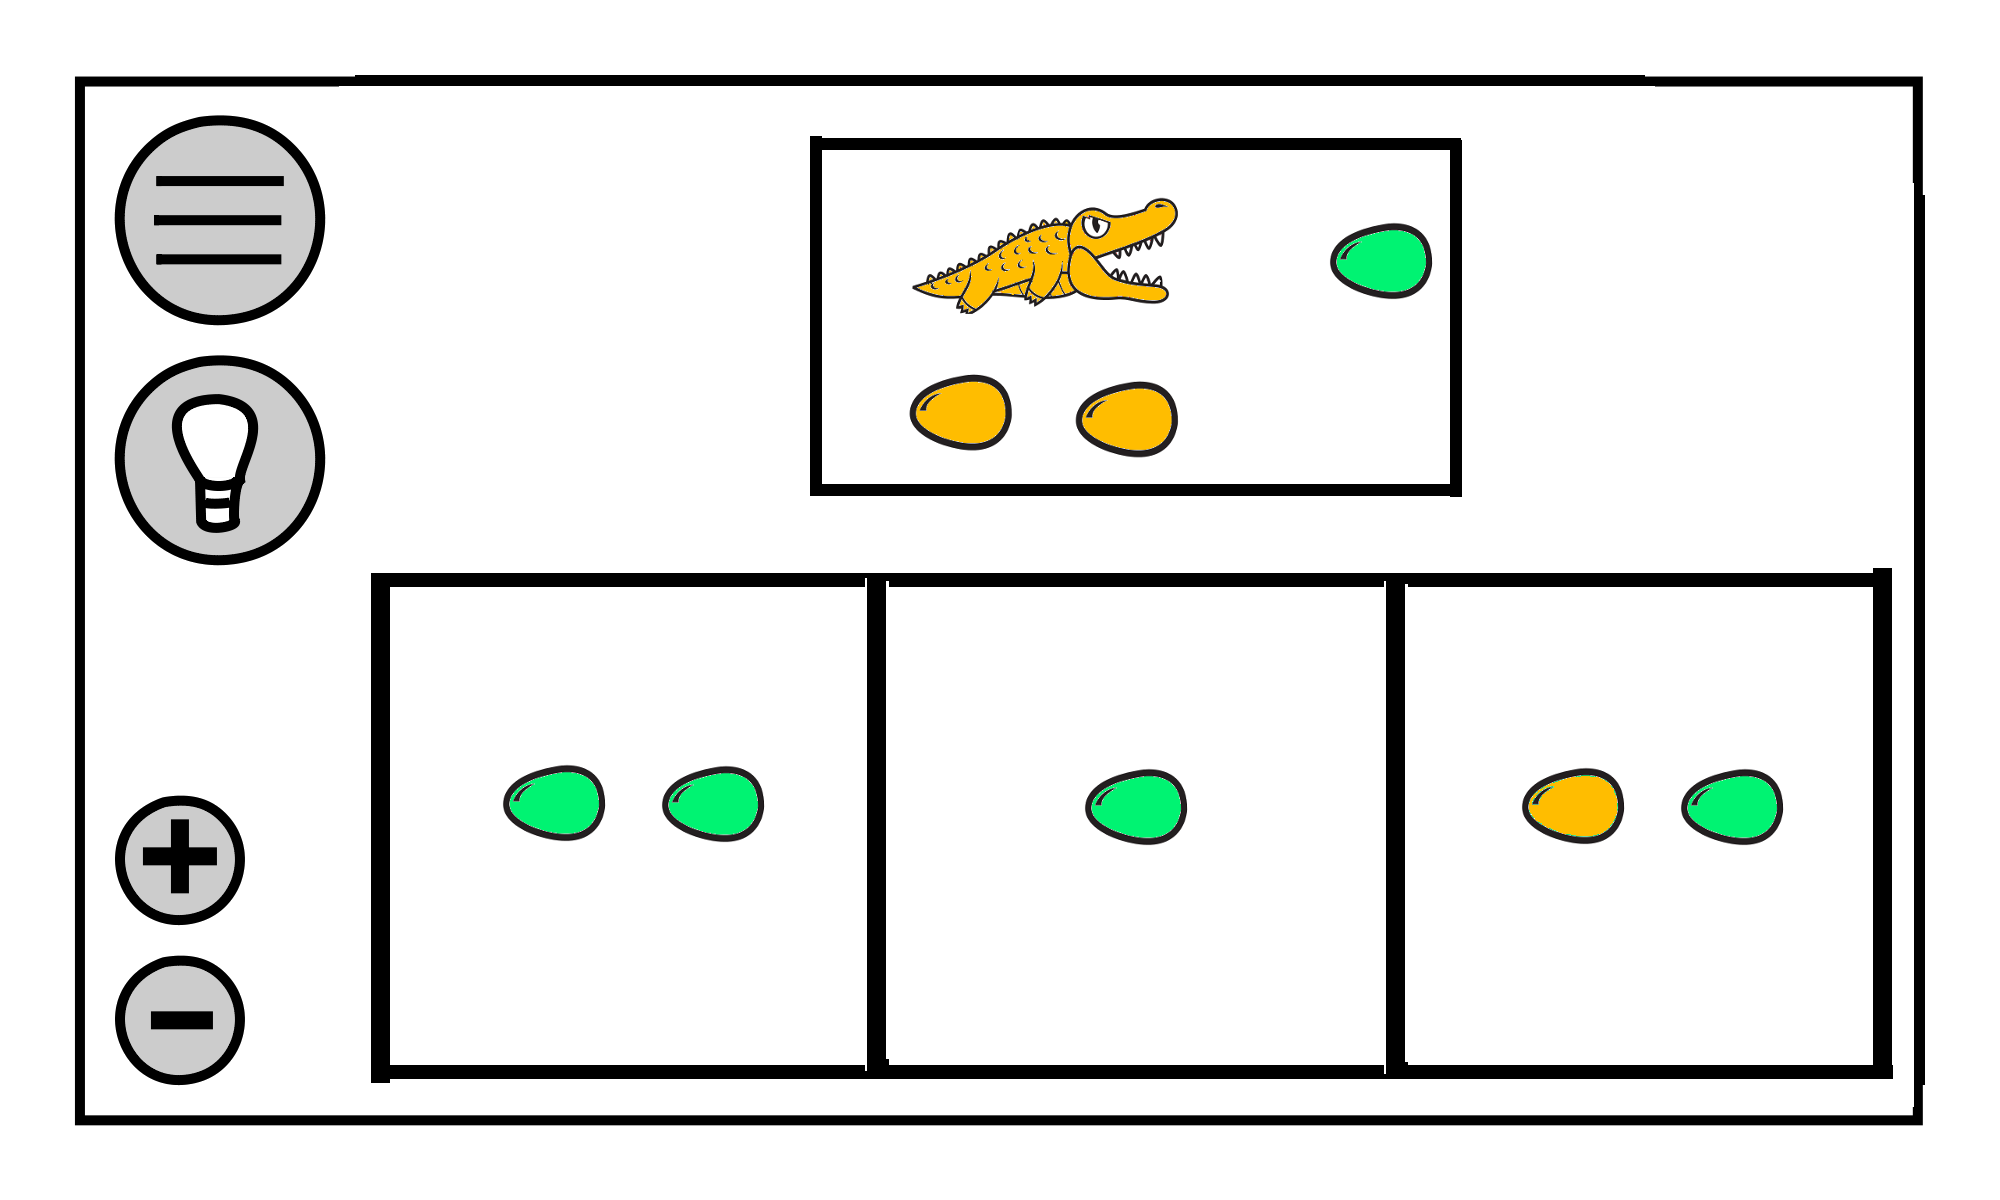
\includegraphics[height=\textheight]{level_choice.png}
\end{frame}
\begin{frame}
	\frametitle{Färbelevel}
	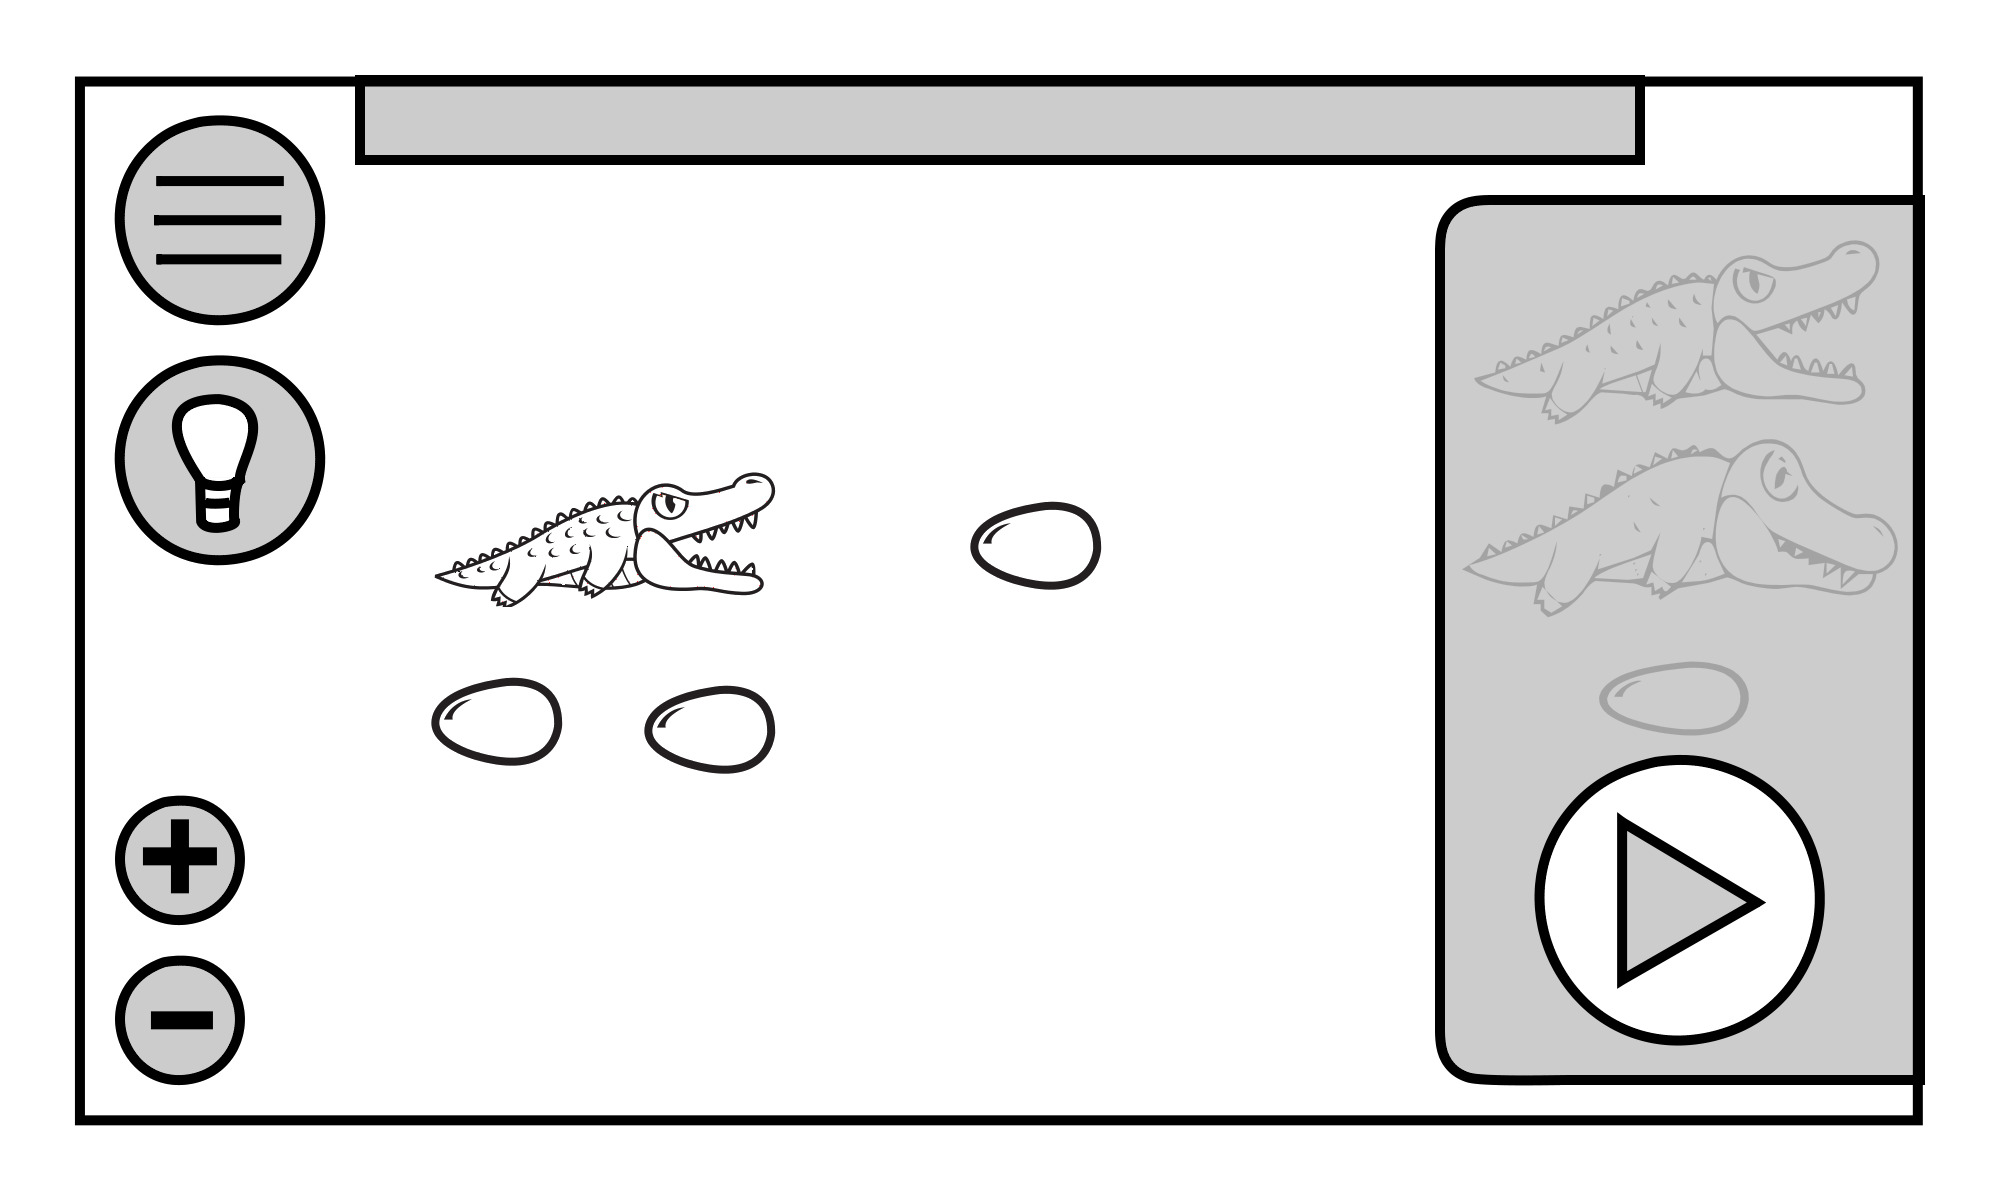
\includegraphics[height=\textheight]{level_white.png}
\end{frame}
\begin{frame}
	\frametitle{Endkonstellation}
	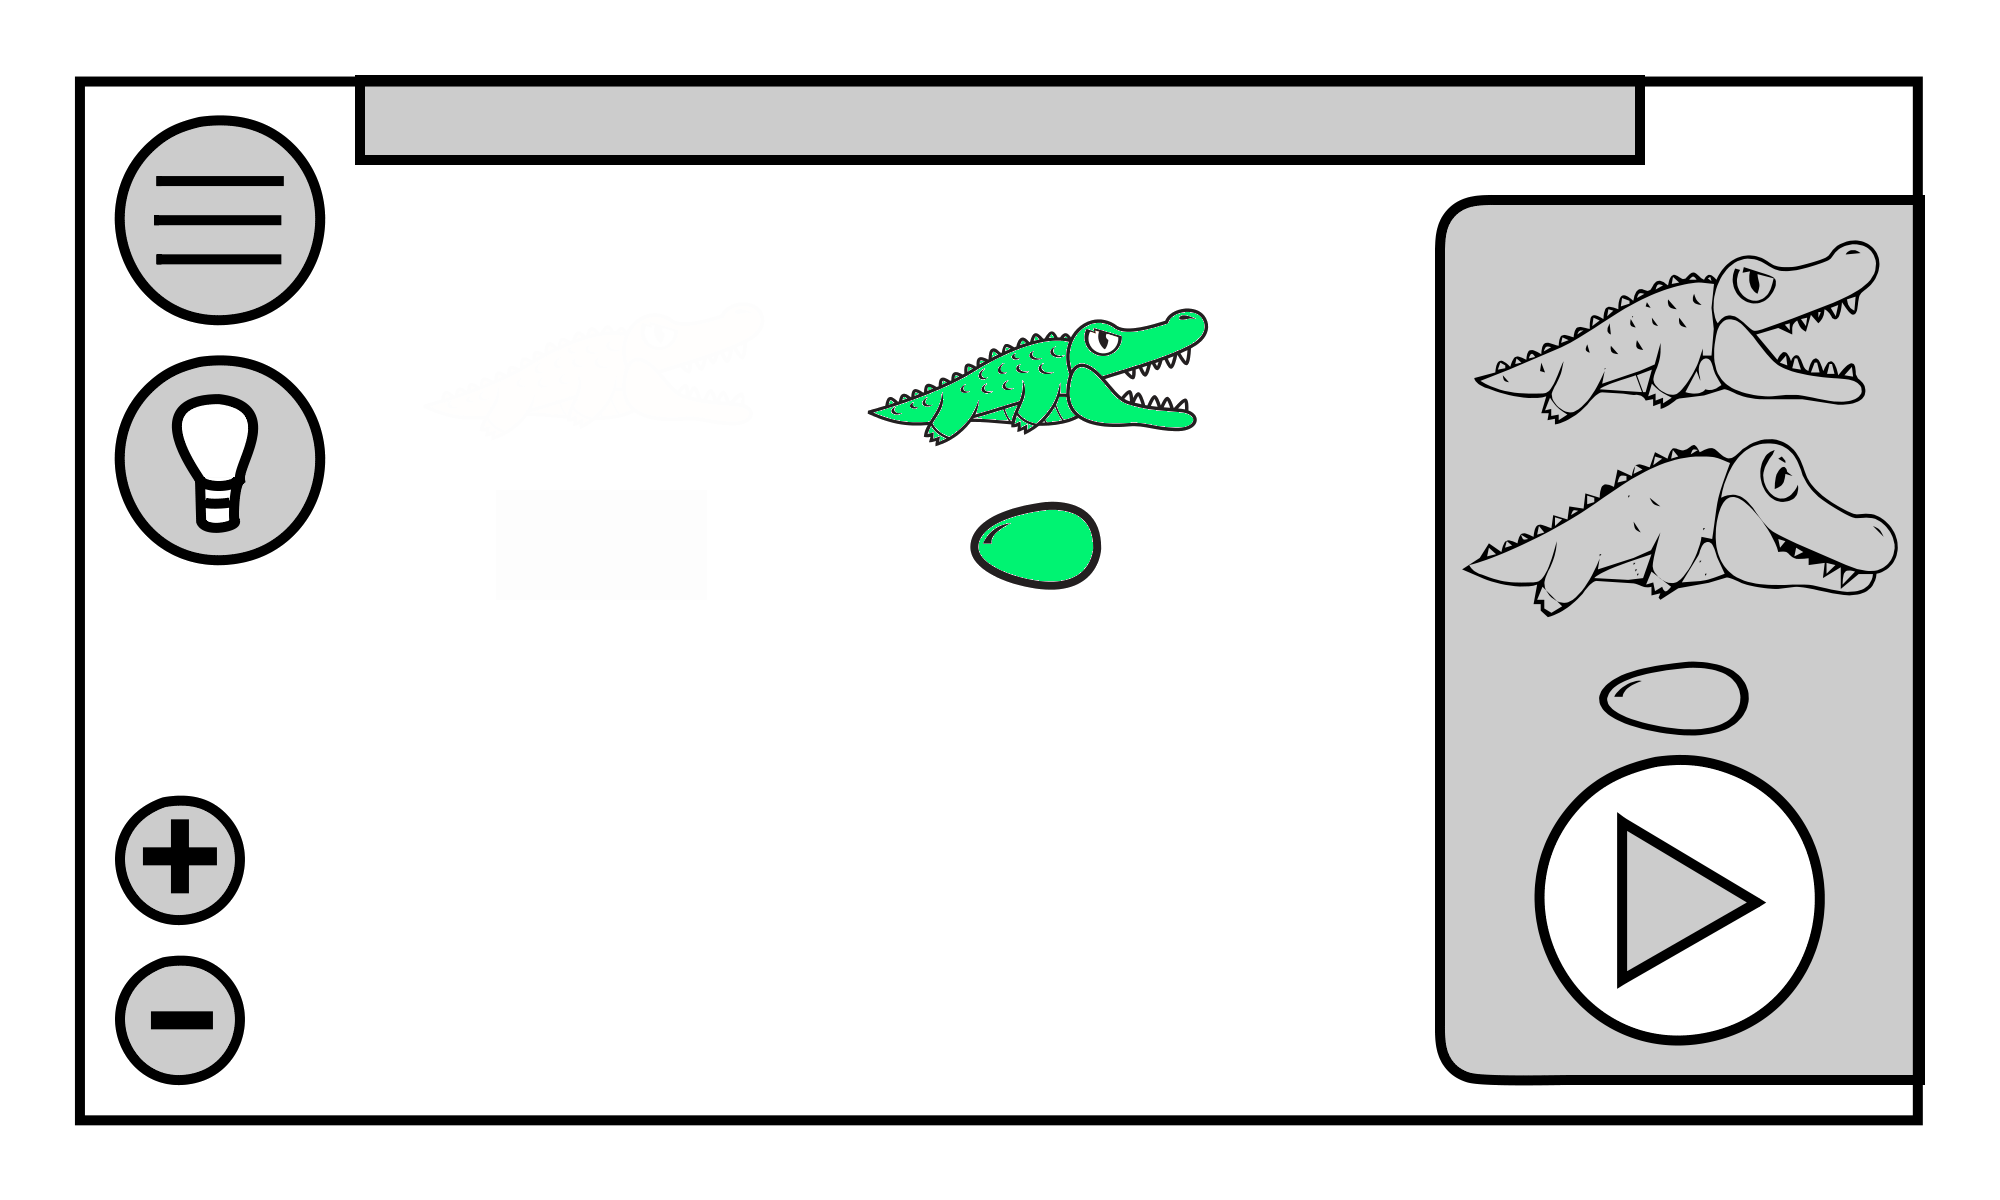
\includegraphics[height=\textheight]{level_end.png}
\end{frame}
\begin{frame}
	\frametitle{Farbauswahl}
	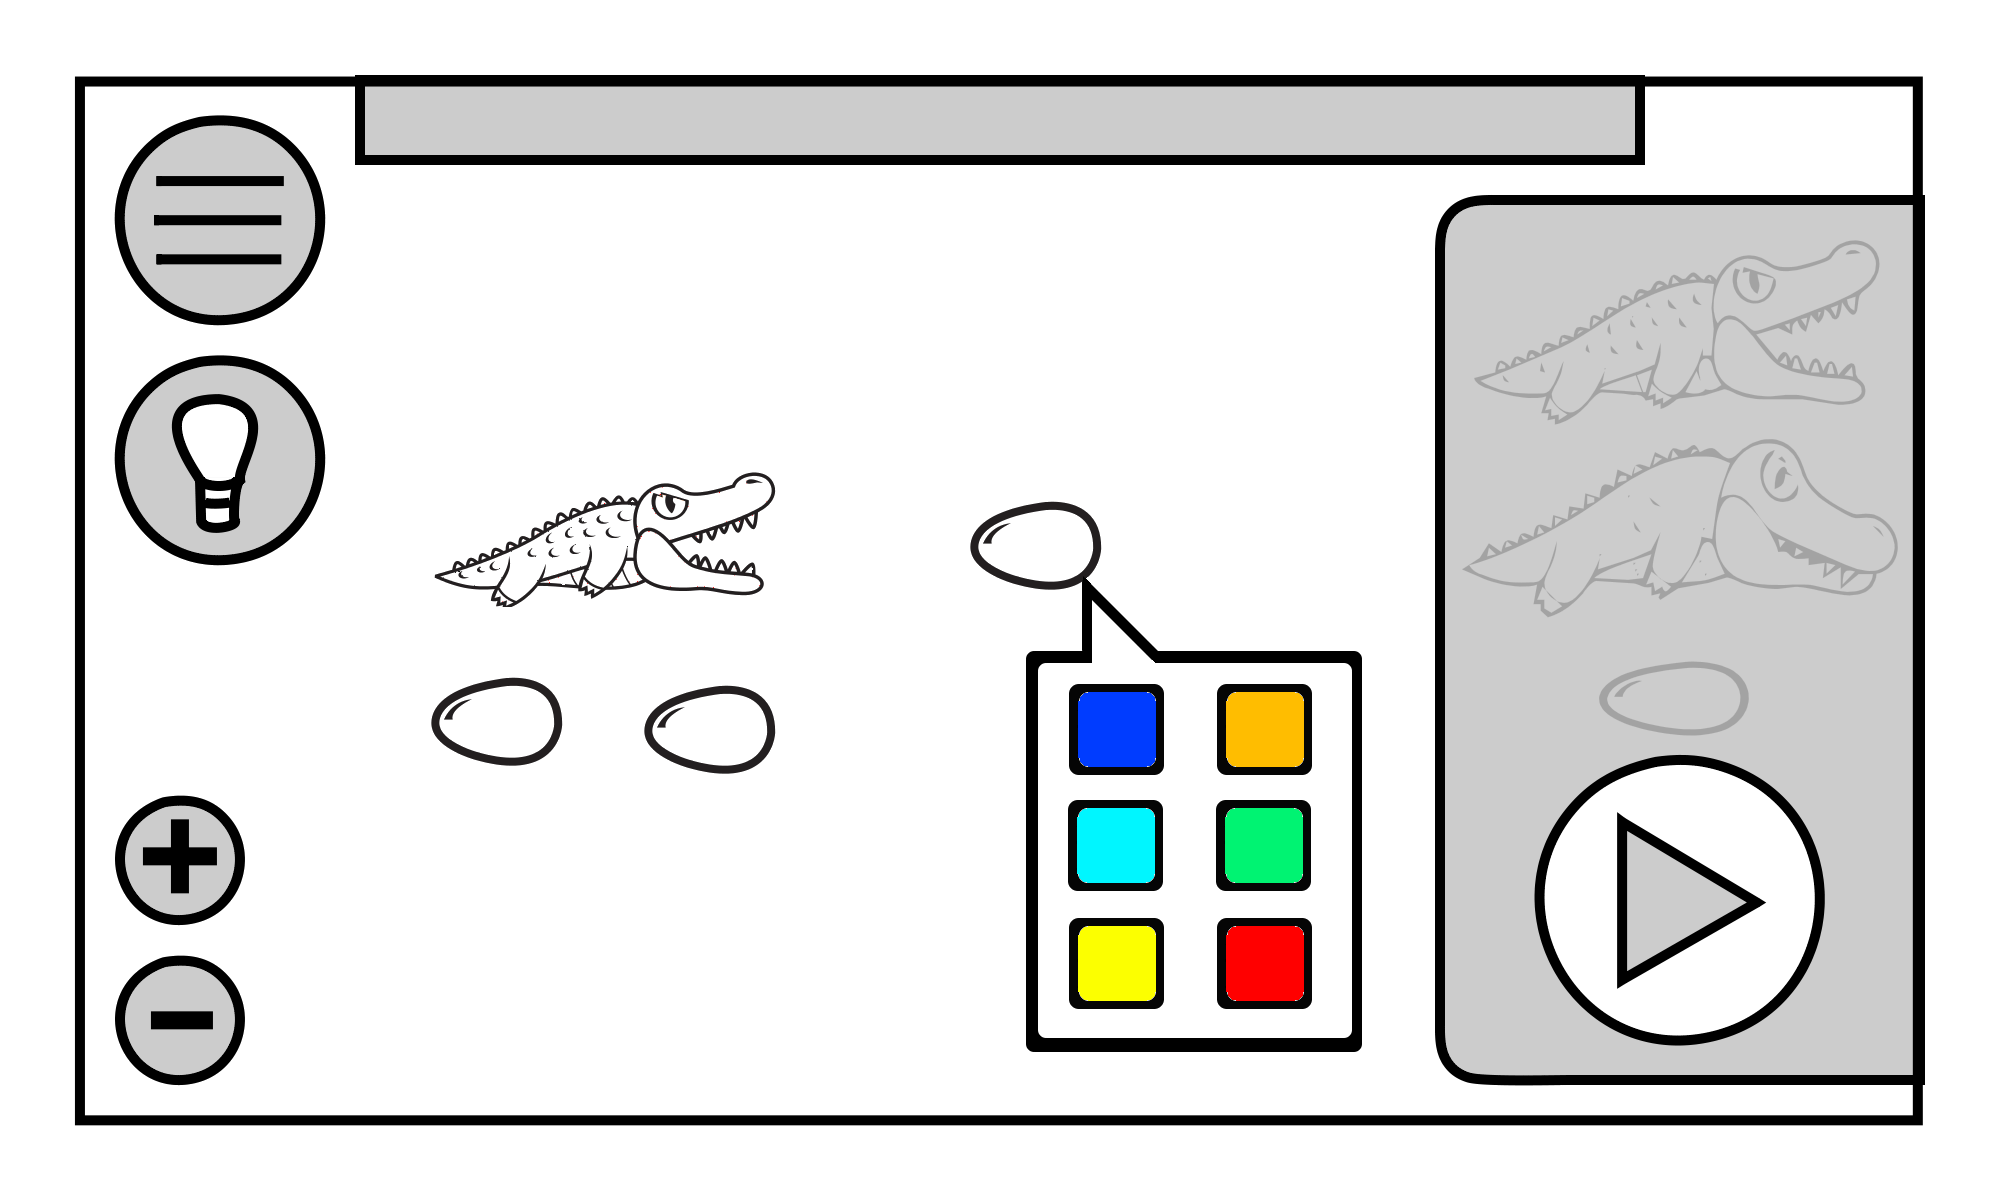
\includegraphics[height=\textheight]{level_color.png}
\end{frame}
\begin{frame}
	\frametitle{Färbelevel}
	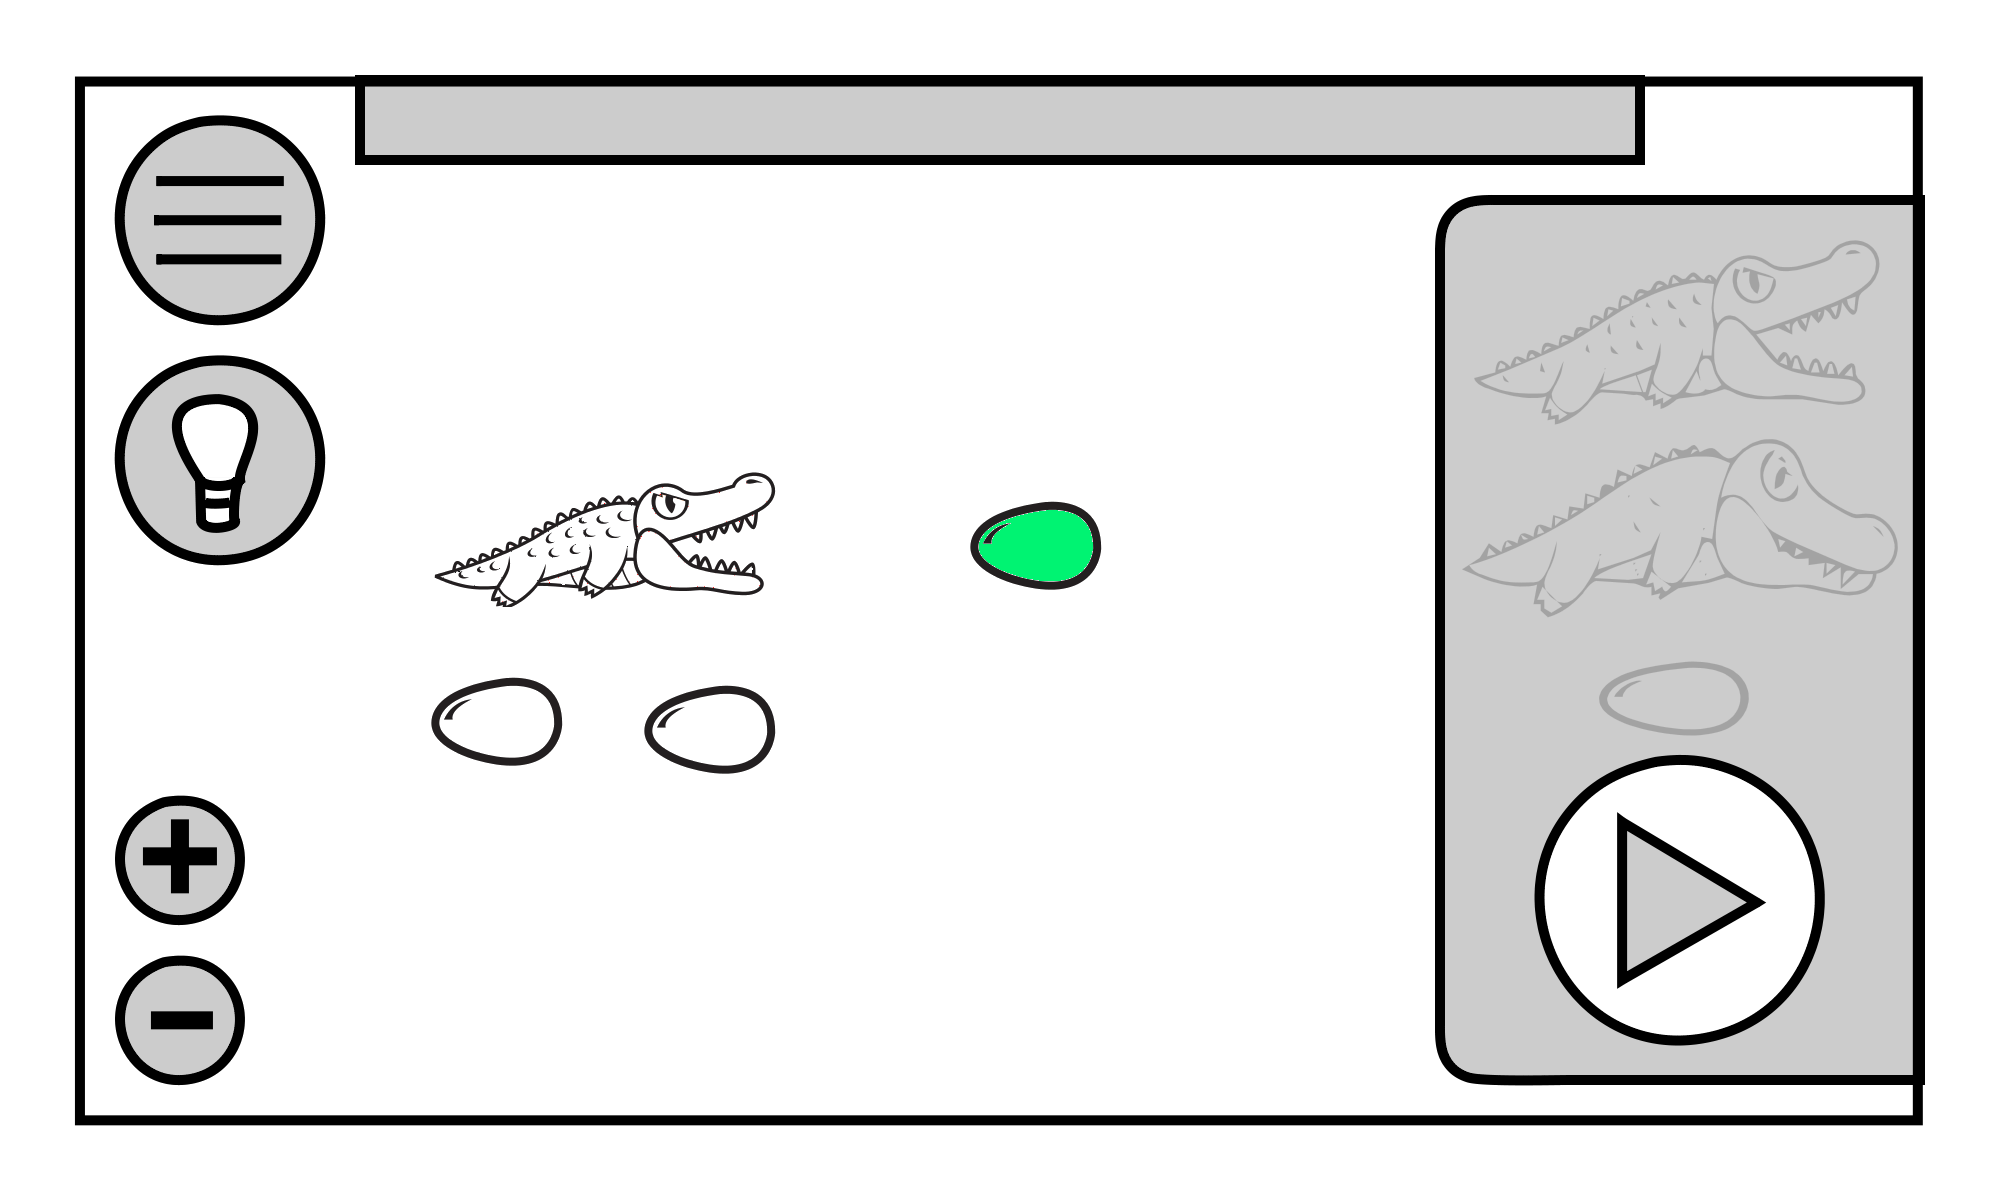
\includegraphics[height=\textheight]{level_colored_egg.png}
\end{frame}
\begin{frame}
	\frametitle{Einfügelevel}
	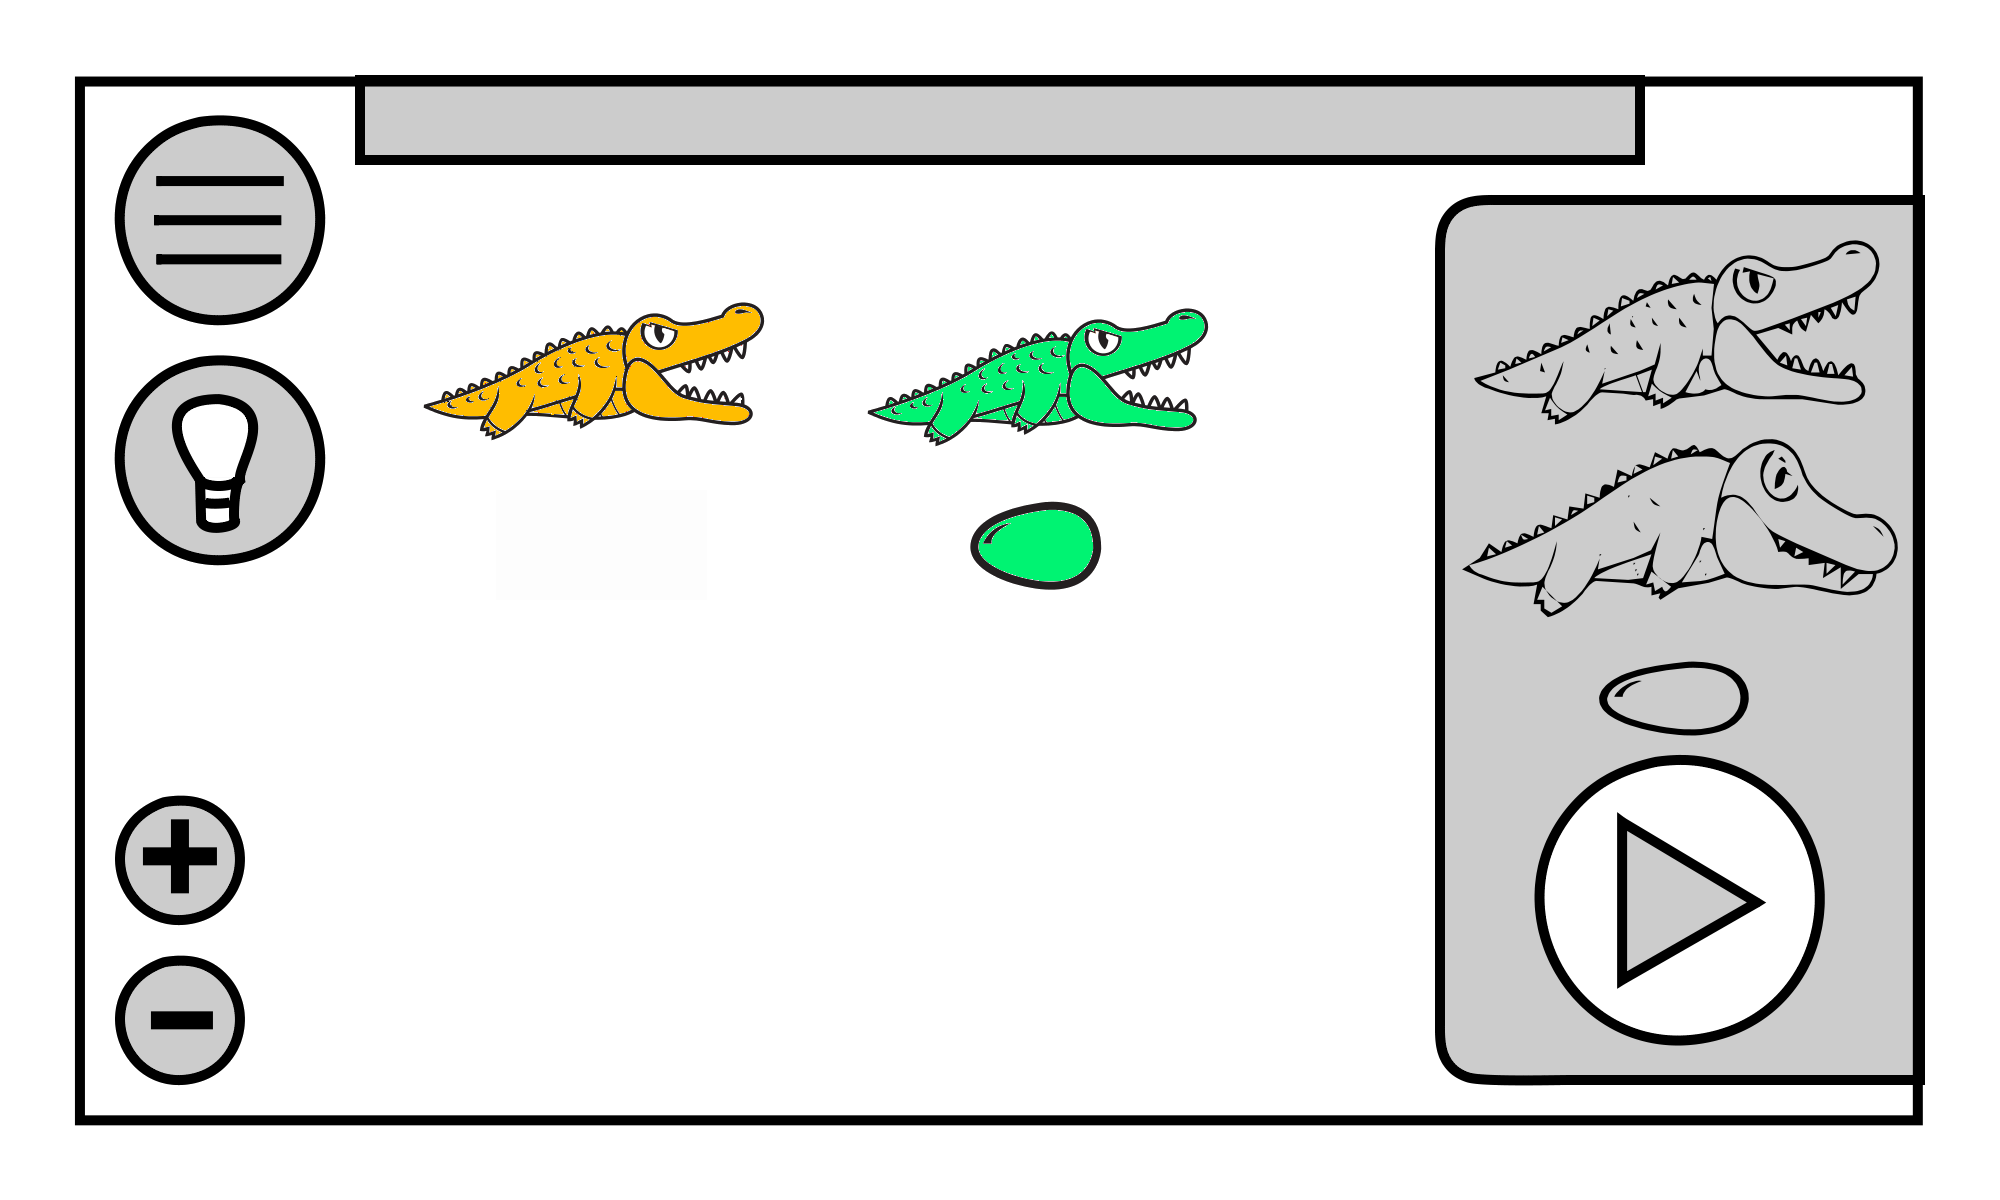
\includegraphics[height=\textheight]{level_start.png}
\end{frame}
\begin{frame}
	\frametitle{Einfügelevel}
	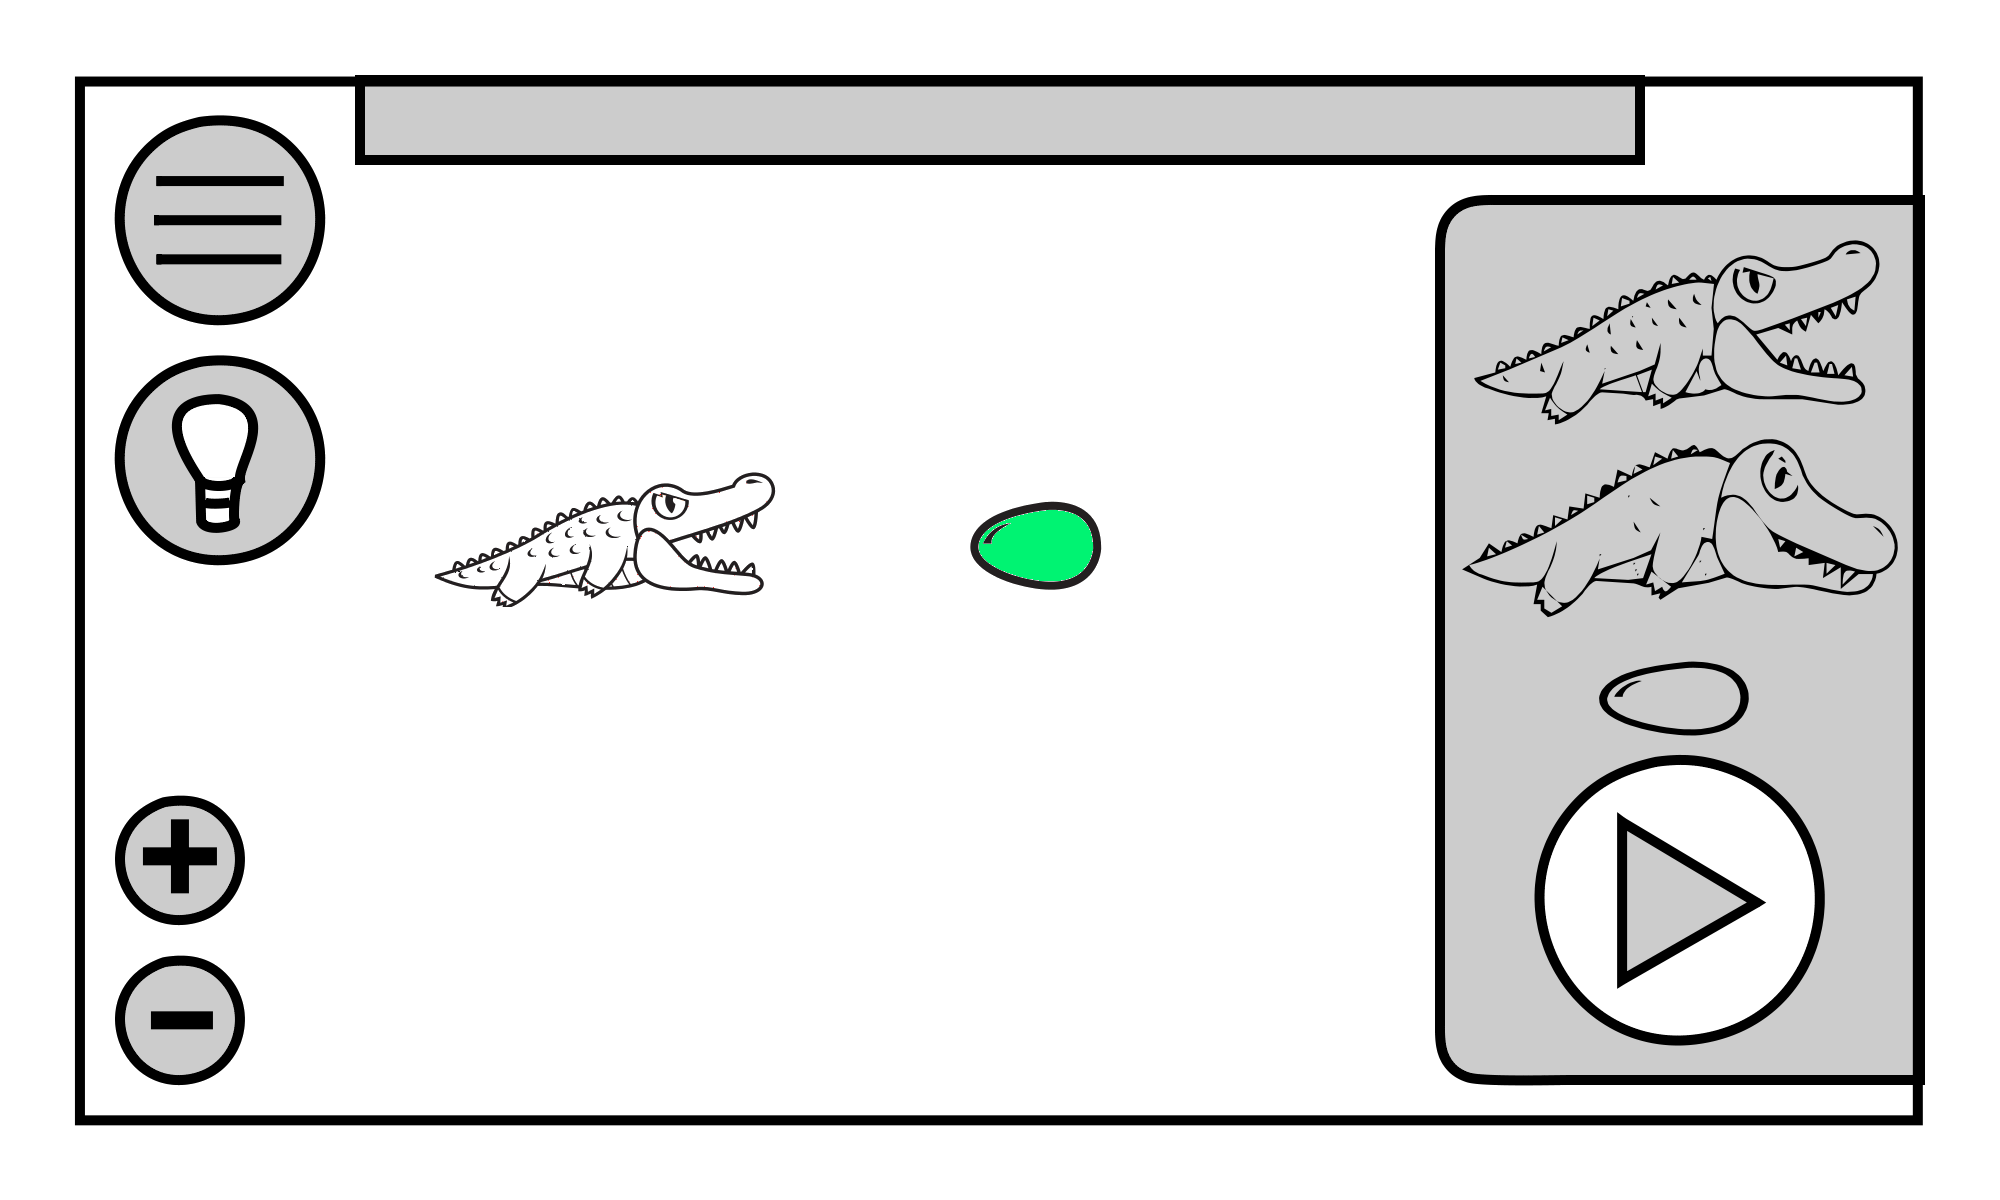
\includegraphics[height=\textheight]{level_croc.png}
\end{frame}
\begin{frame}
	\frametitle{Einfügelevel}
	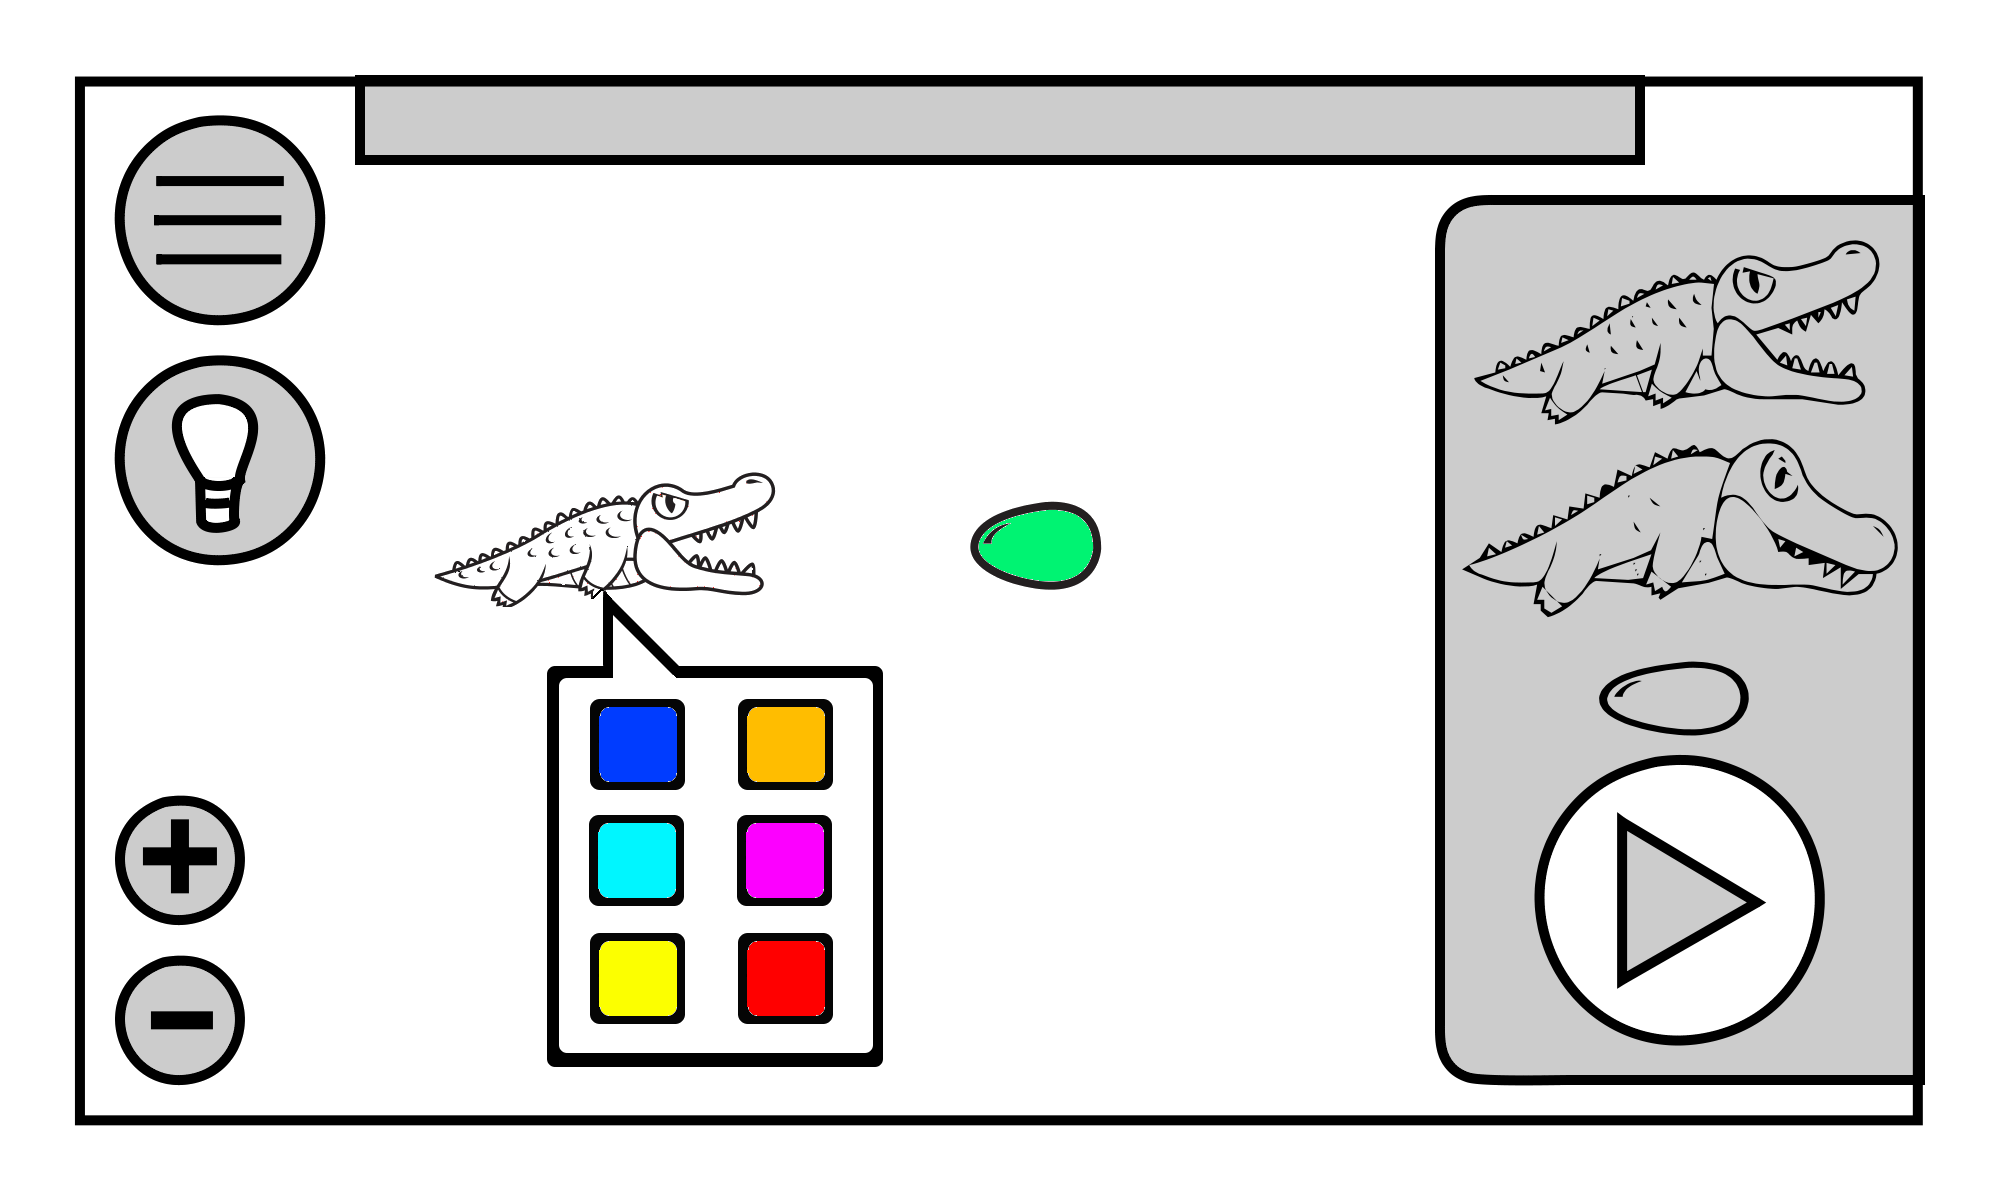
\includegraphics[height=\textheight]{level_color_purple.png}
\end{frame}
\begin{frame}
	\frametitle{Einfügelevel}
	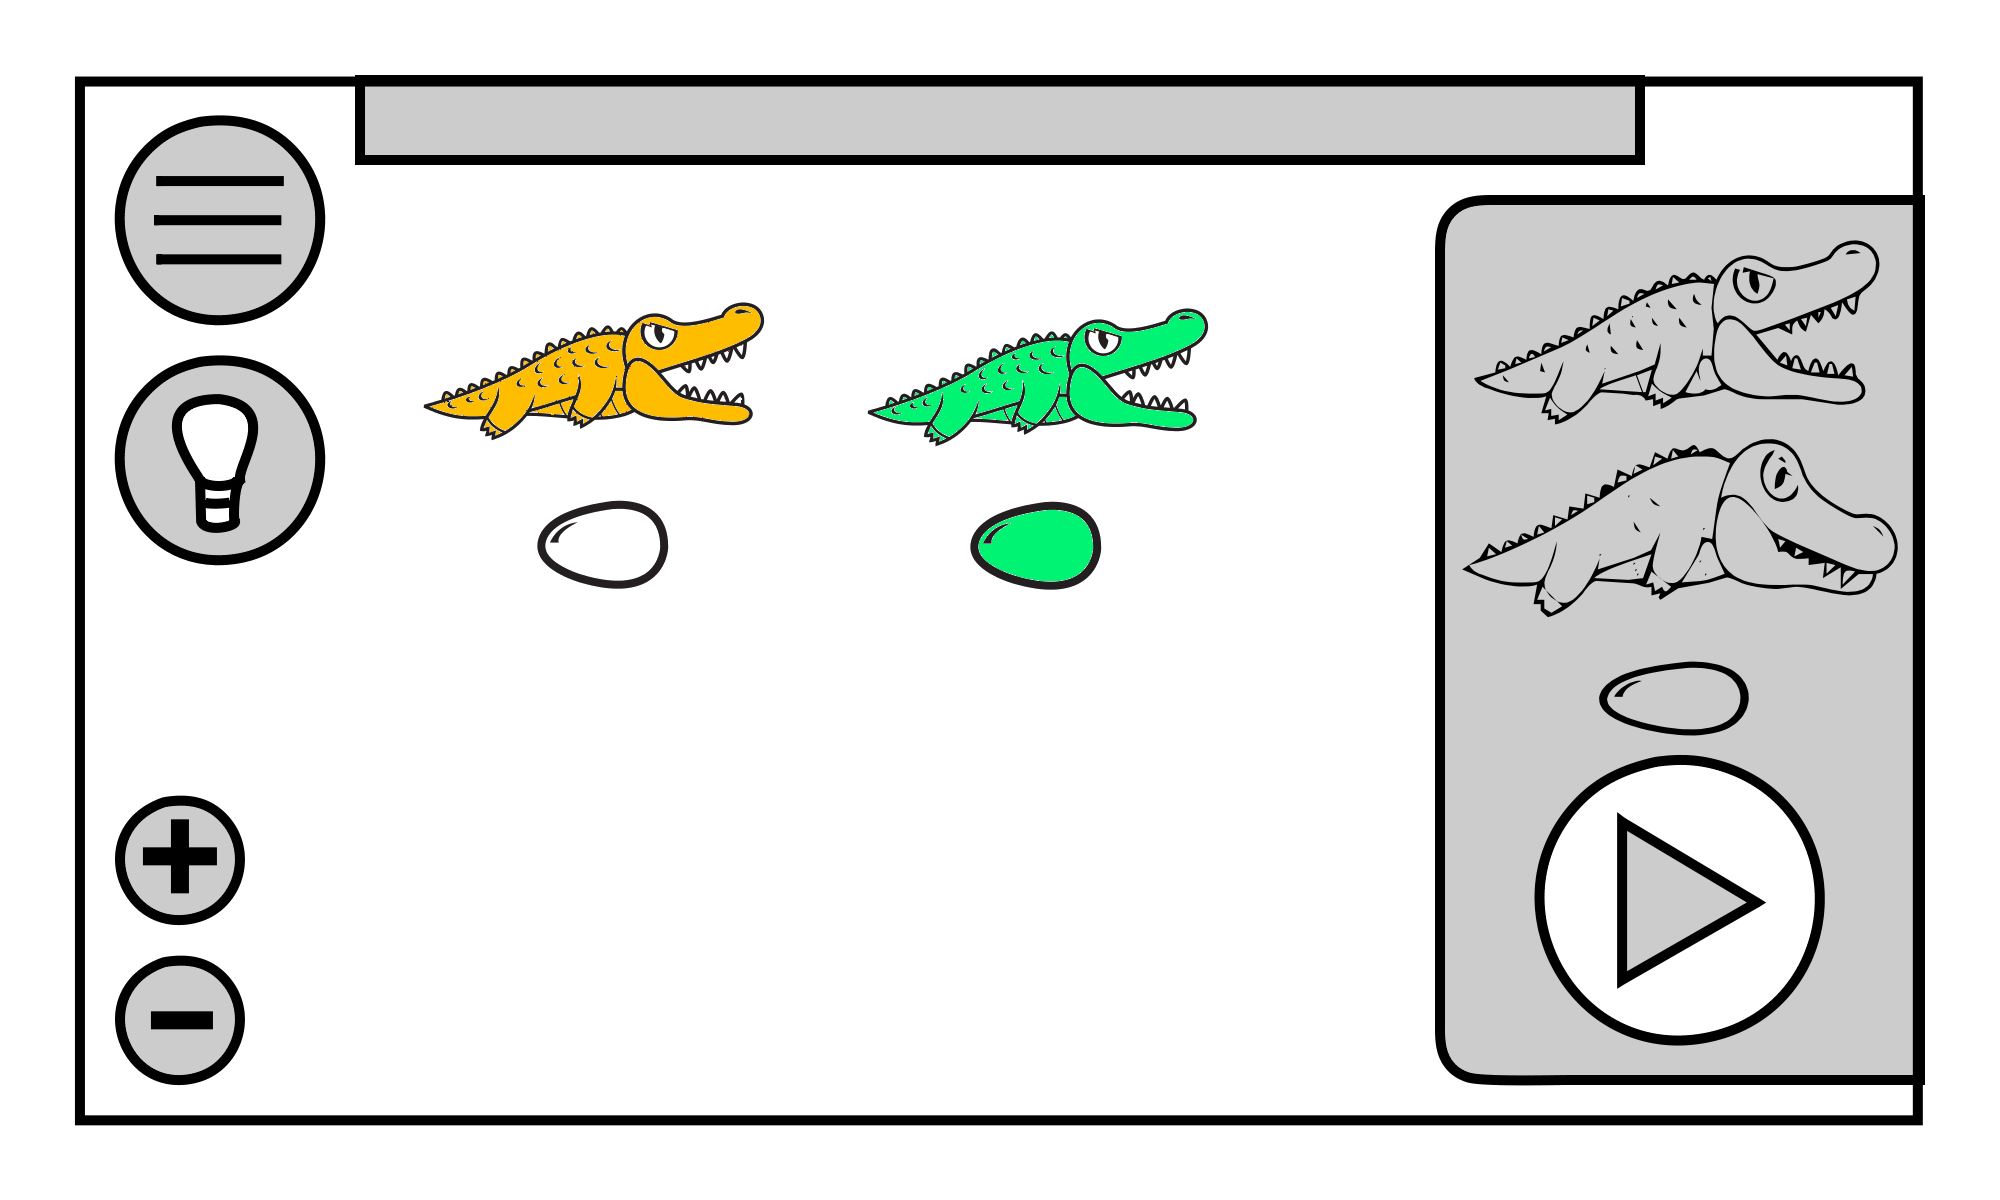
\includegraphics[height=\textheight]{level_colored_croc.png}
\end{frame}
\begin{frame}
	\frametitle{Einfügelevel}
	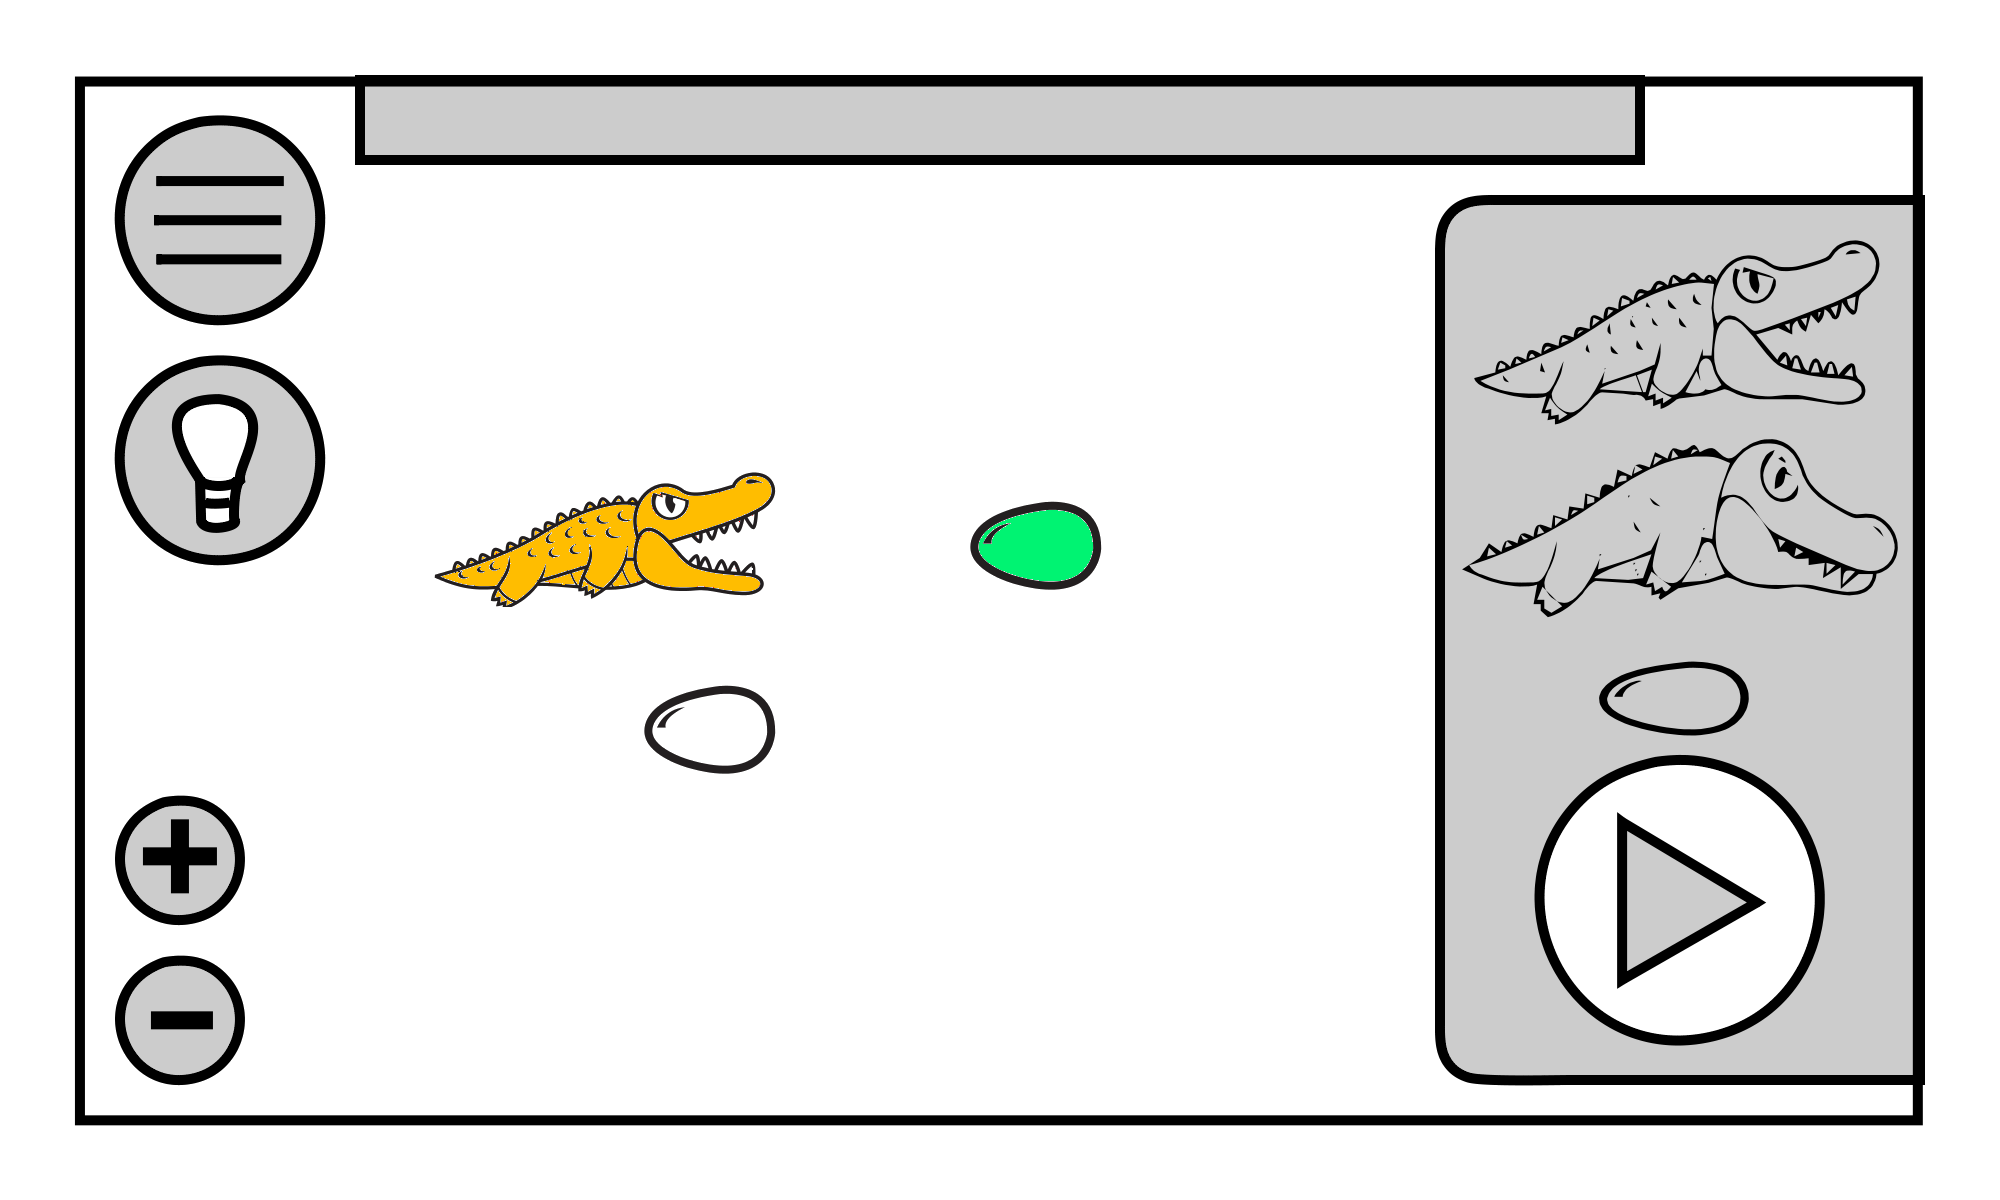
\includegraphics[height=\textheight]{level_colored_croc0.png}
\end{frame}
\begin{frame}
	\frametitle{Einfügelevel}
	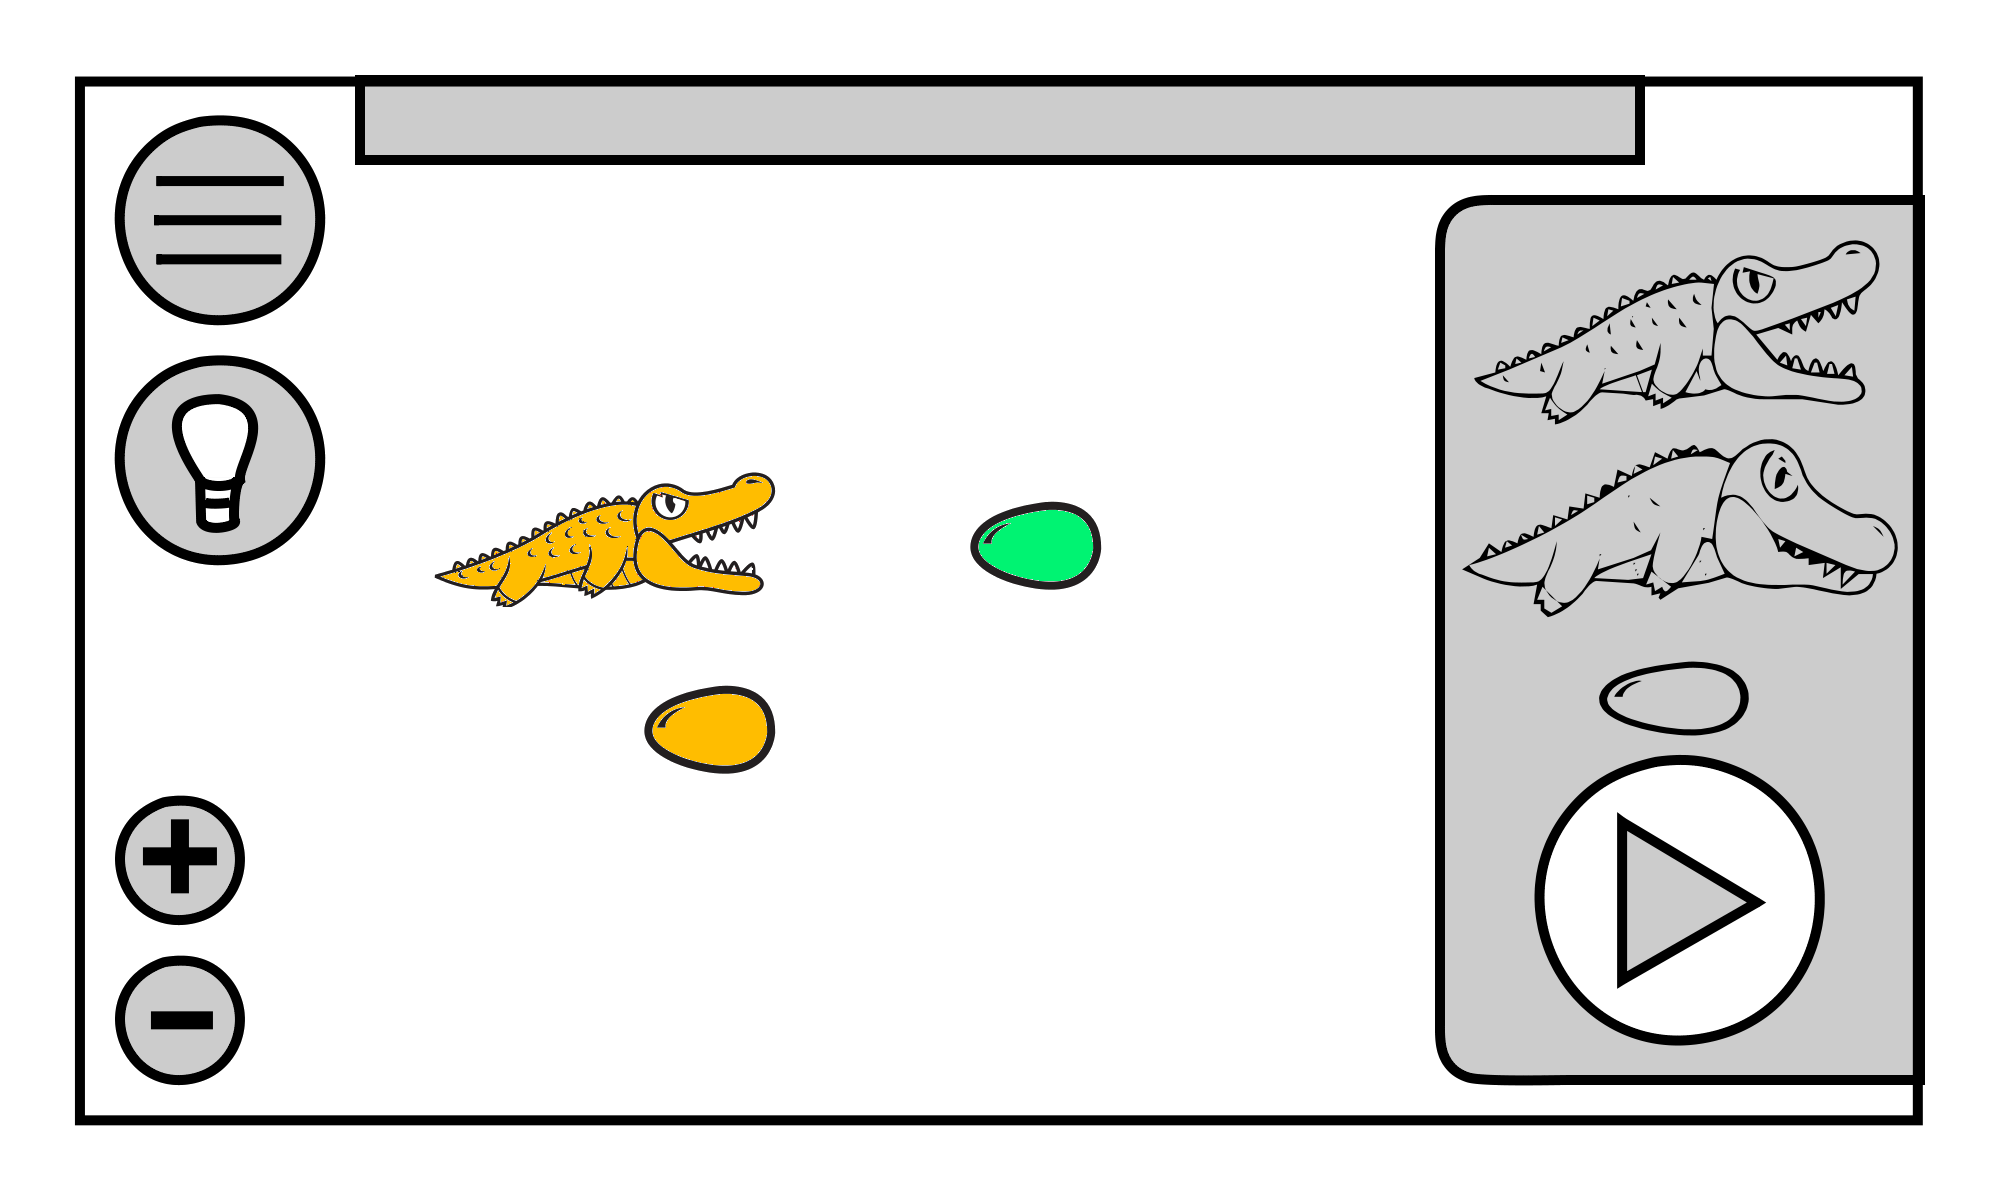
\includegraphics[height=\textheight]{level_colored_croc01.png}
\end{frame}
\begin{frame}
	\frametitle{Einfügelevel}
	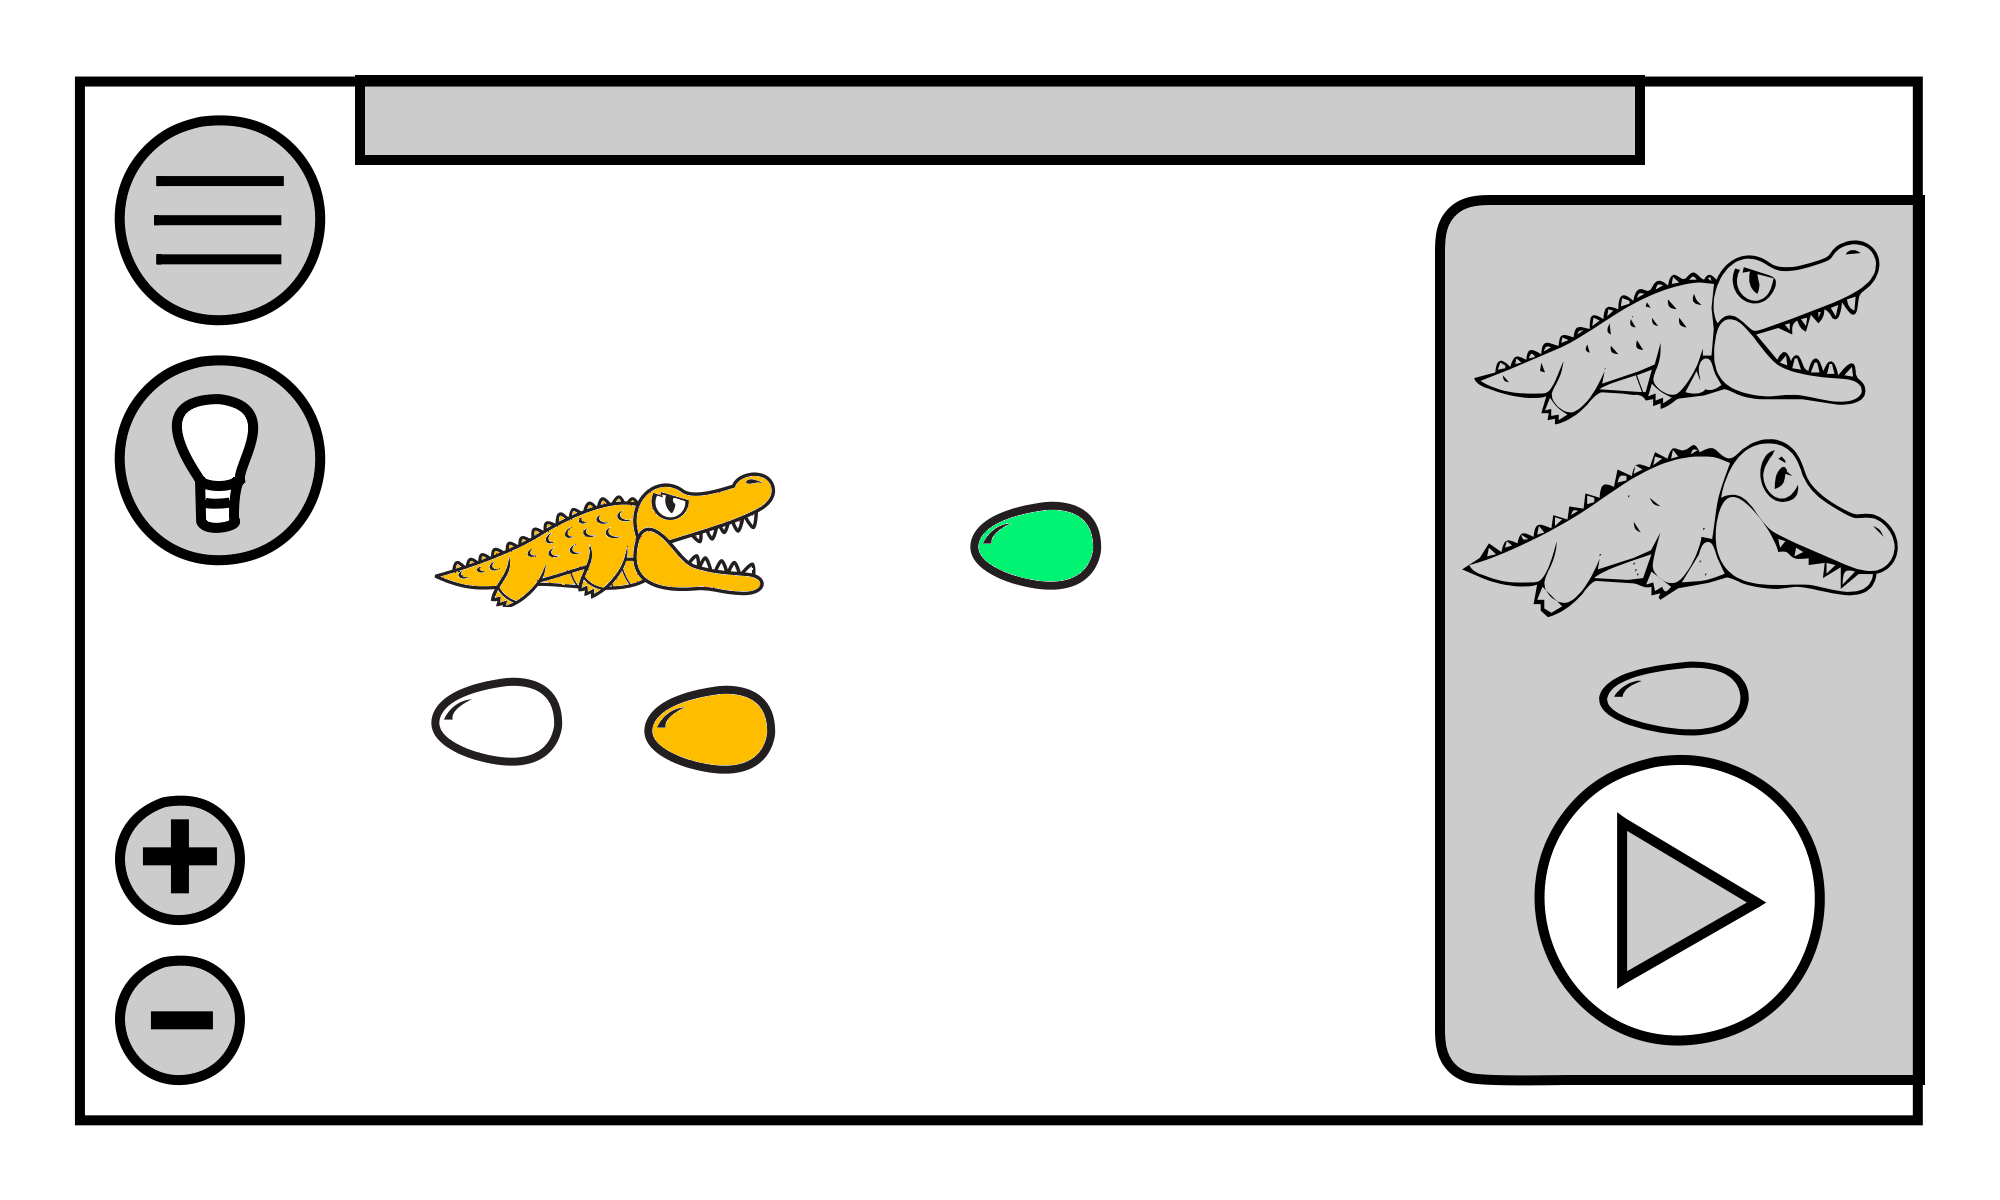
\includegraphics[height=\textheight]{level_colored_croc1.png}
\end{frame}
\begin{frame}
	\frametitle{Einfügelevel}
	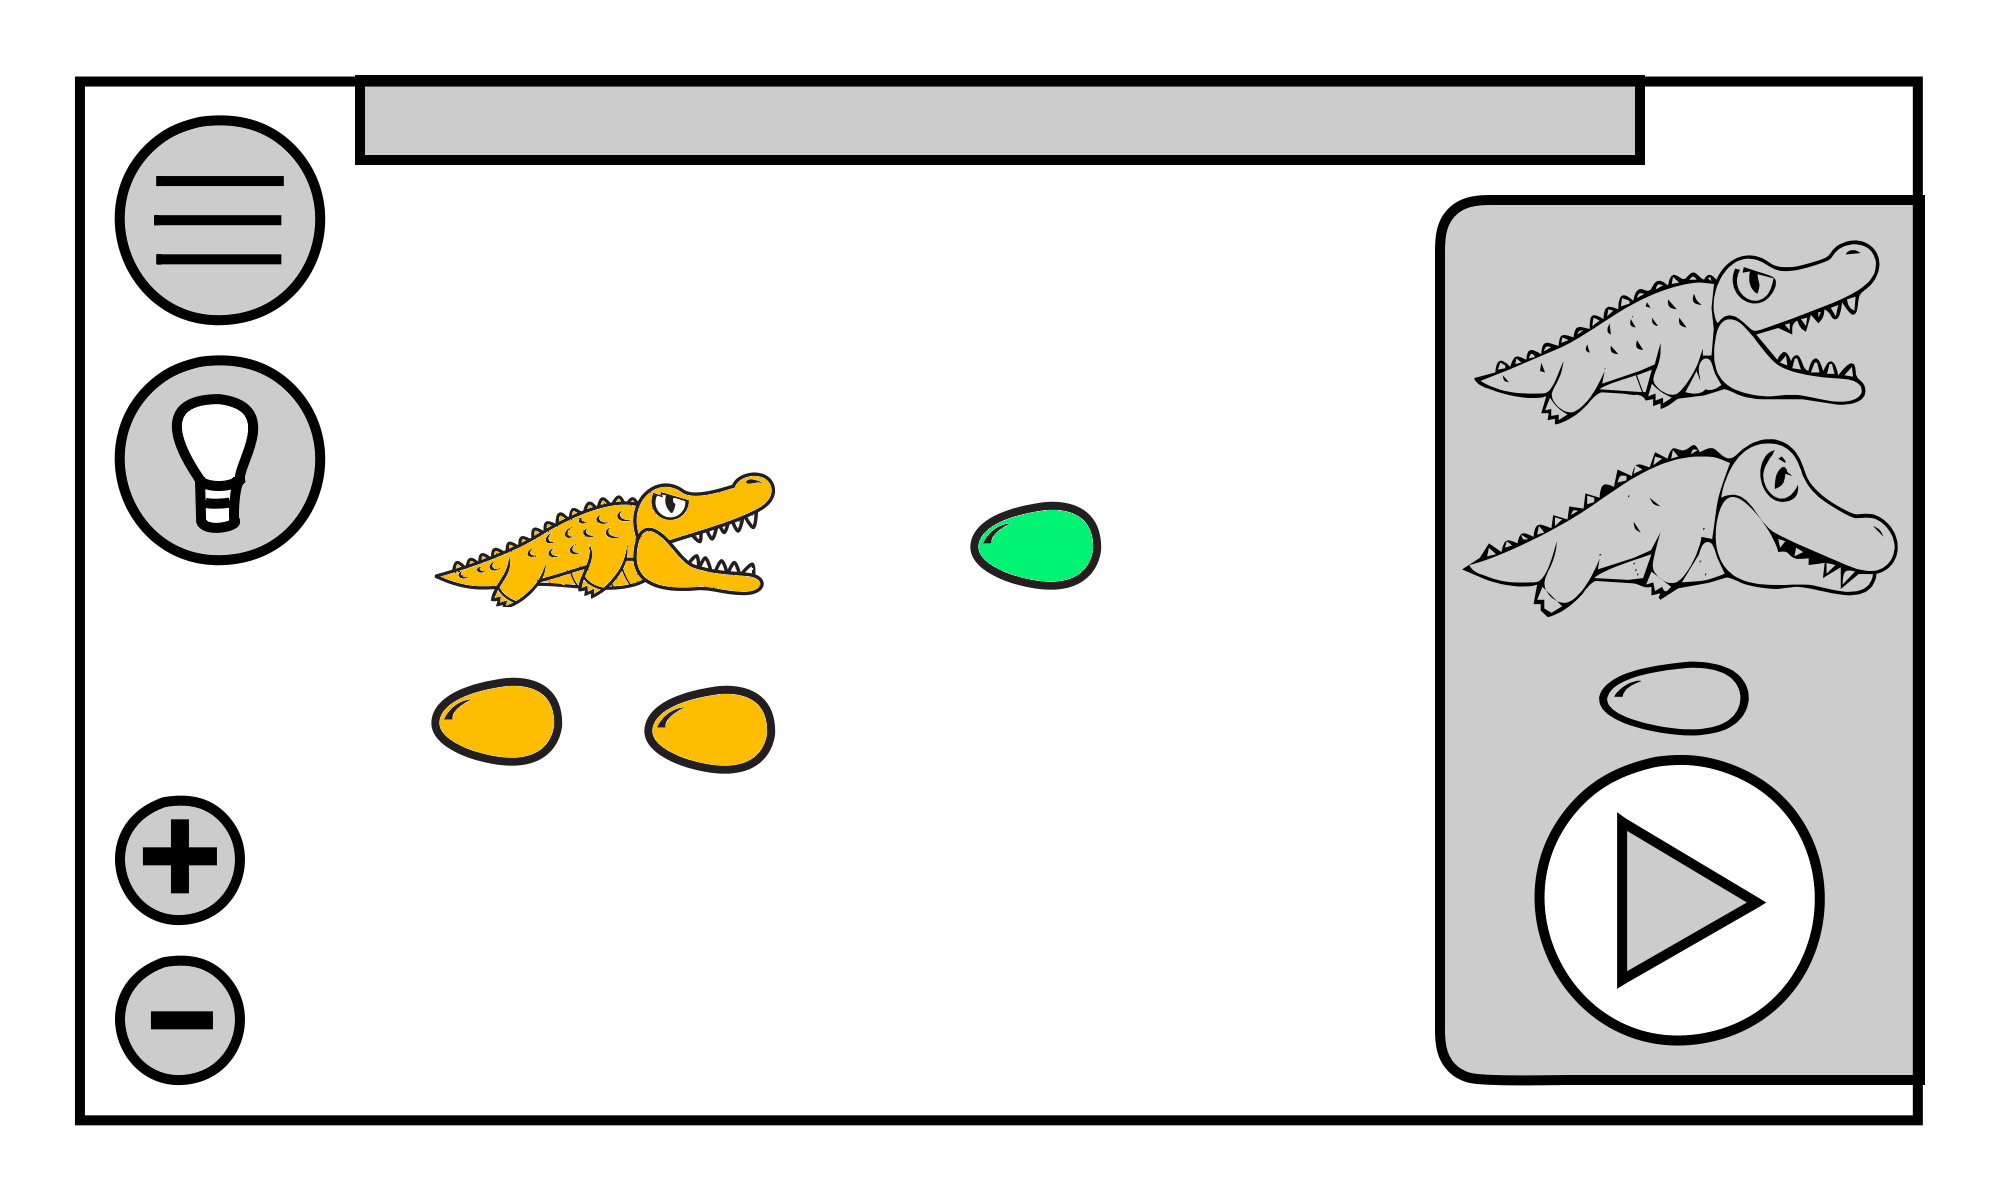
\includegraphics[height=\textheight]{level_colored_croc2.png}
\end{frame}
\begin{frame}
	\frametitle{Simulationsmodus}
	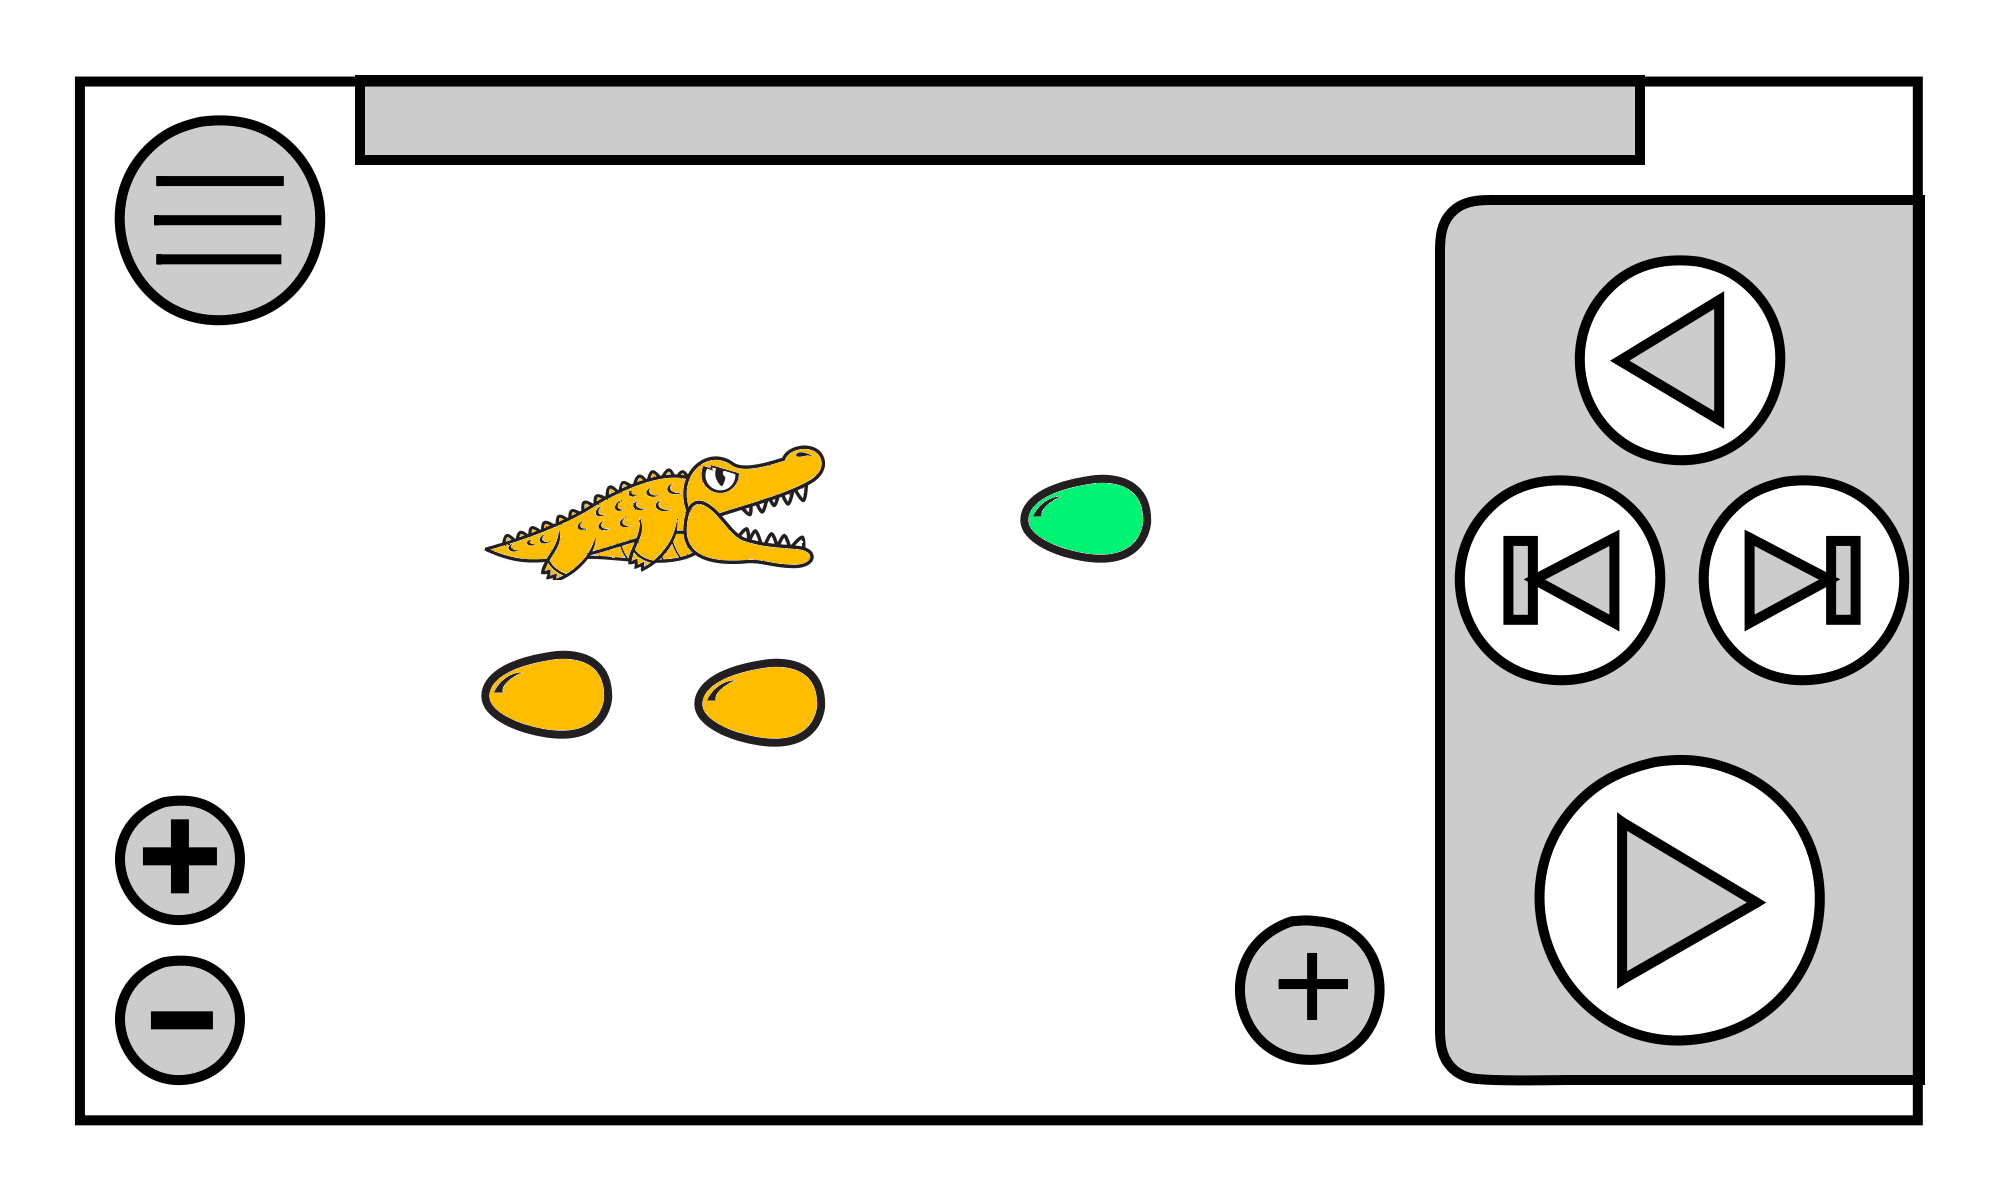
\includegraphics[height=\textheight]{level_simulation_croc.png}
\end{frame}
\begin{frame}
	\frametitle{Simulationsmodus}
	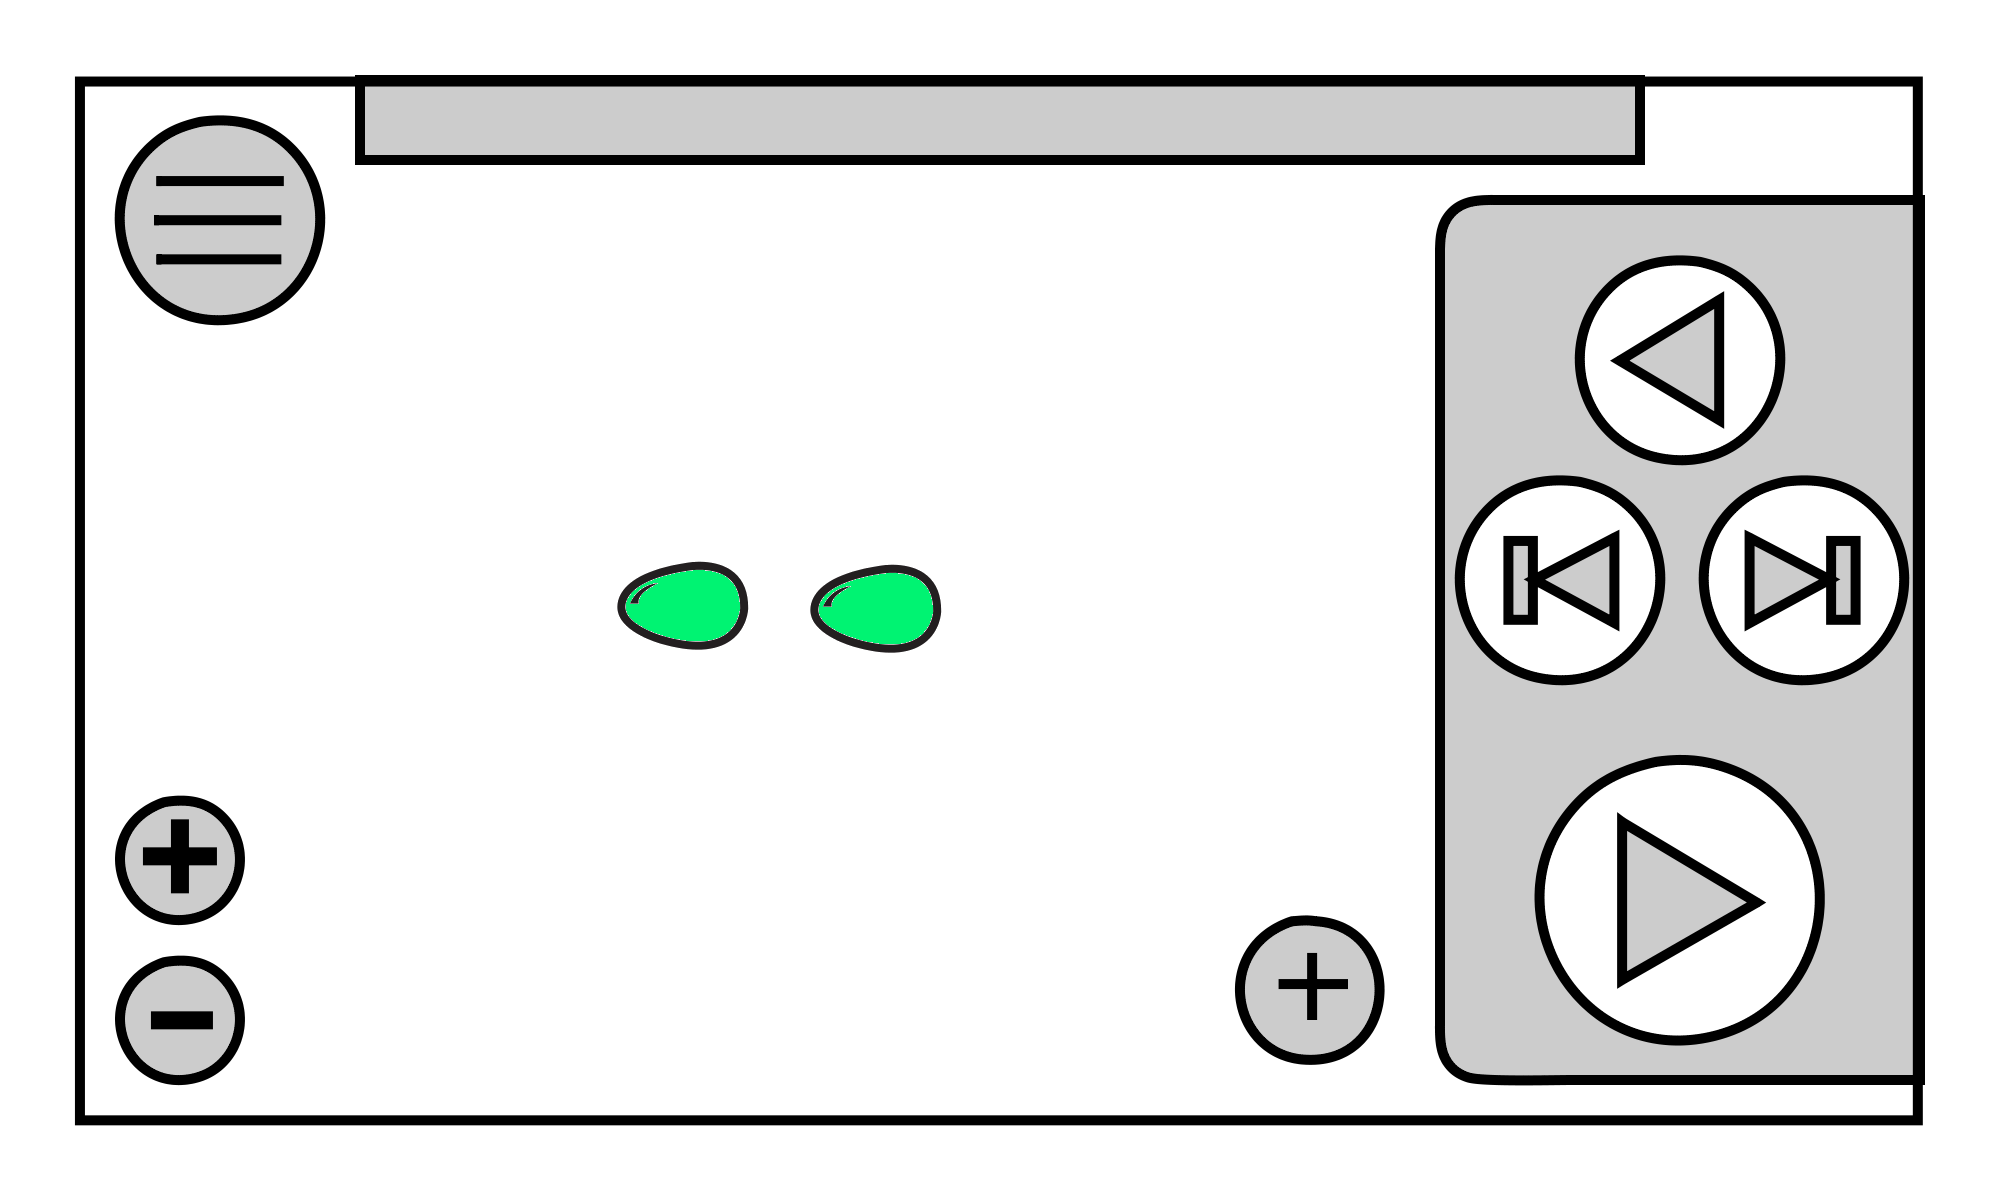
\includegraphics[height=\textheight]{level_simulation_solved.png}
\end{frame}
\begin{frame}
	\frametitle{Achievement unlocked}
	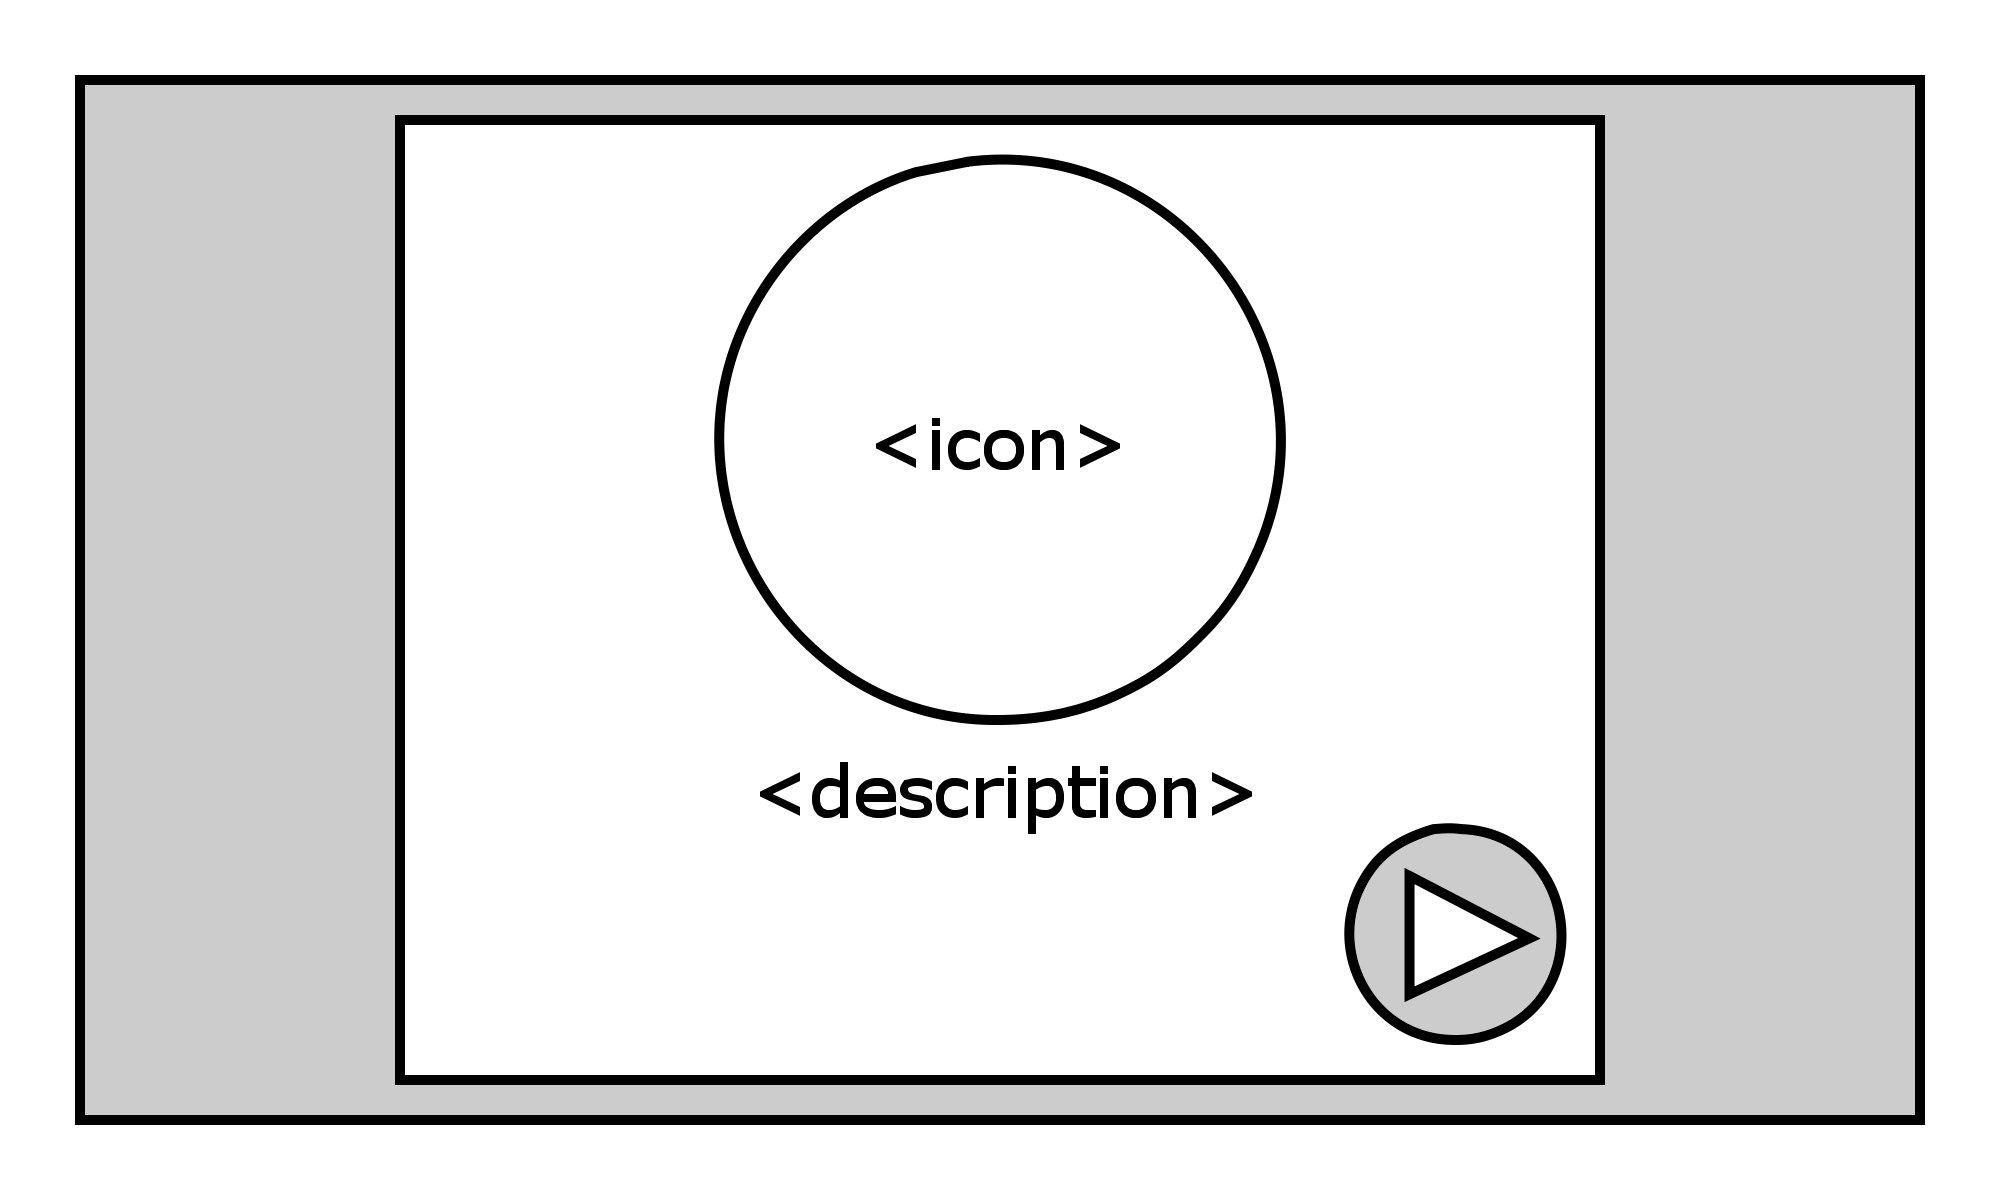
\includegraphics[height=\textheight]{achievement_notification.png}
\end{frame}
\begin{frame}
	\frametitle{Achievementmenü}
	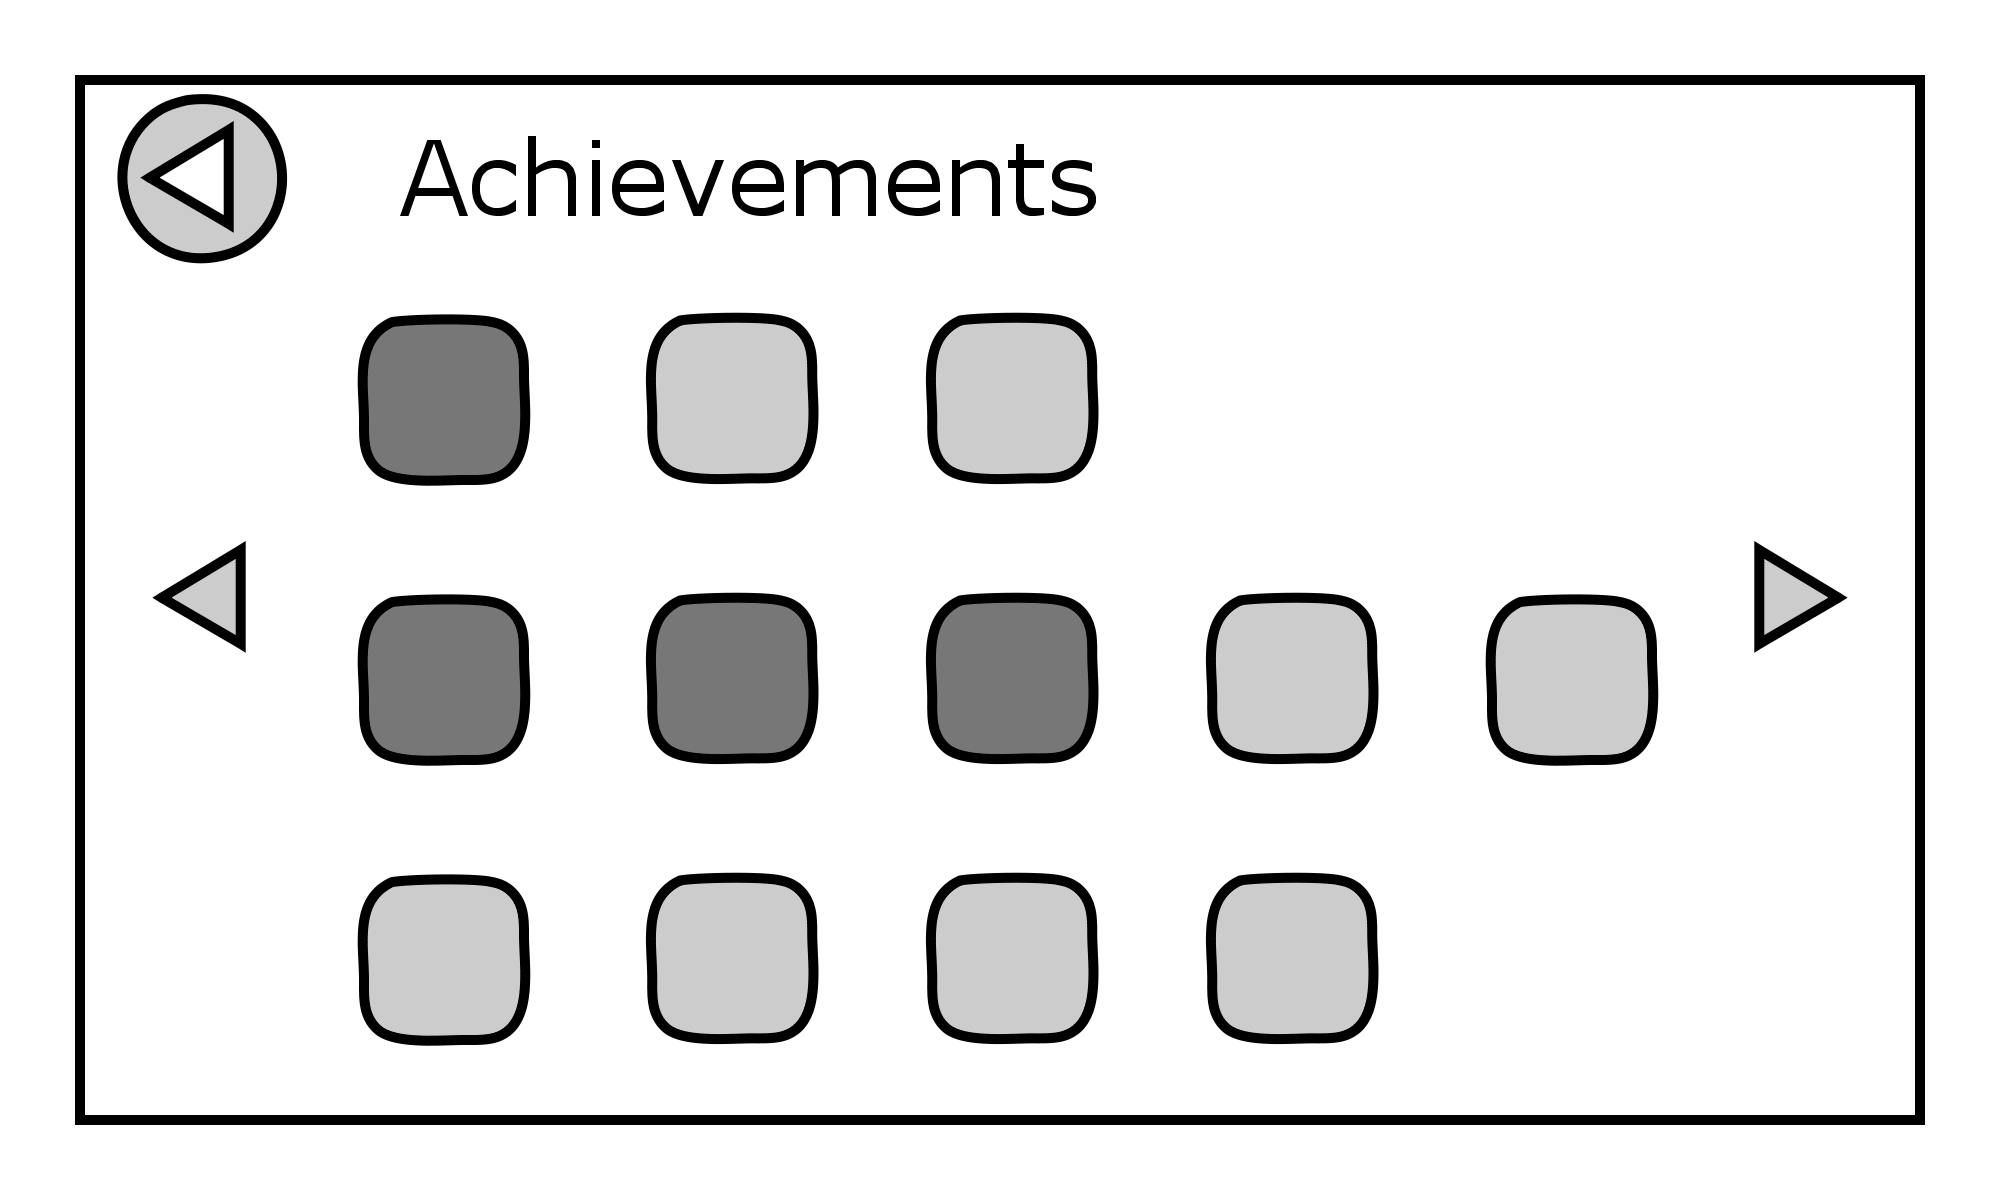
\includegraphics[height=\textheight]{achievements.png}
\end{frame}
\begin{frame}
	\frametitle{Statistiken}
	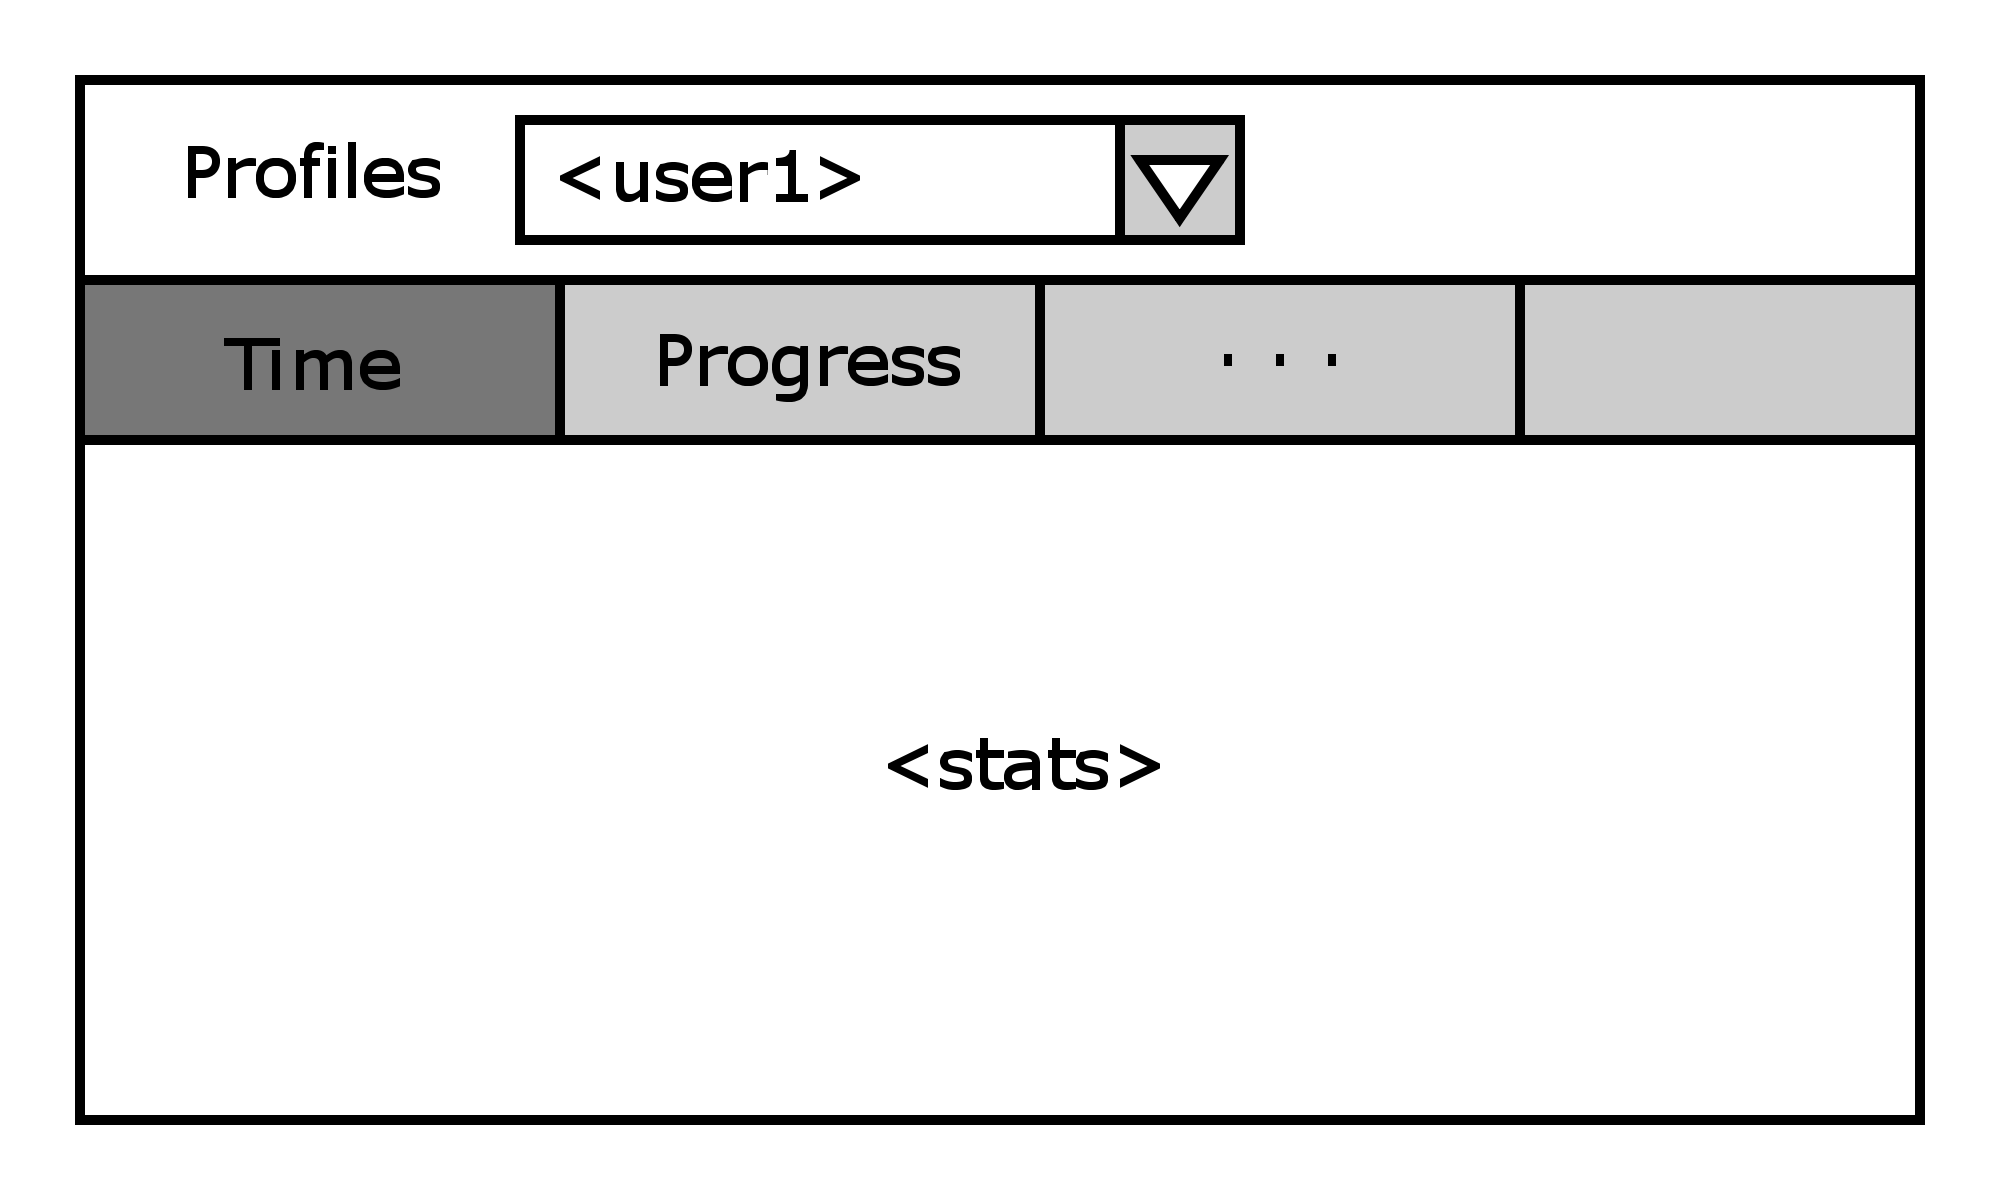
\includegraphics[height=\textheight]{stats.png}
\end{frame}

\end{document}
